%  LaTeX support: latex@mdpi.com
%  For support, please attach all files needed for compiling as well as the log file, and specify your operating system, LaTeX version, and LaTeX editor.

%=================================================================
\documentclass[journal,article,submit,moreauthors,technologies]{Definitions/mdpi}
%\documentclass[journal,article,submit,moreauthors,unicode]{Definitions/mdpi} % For some letters Palatino lacks
%\documentclass[preprints,article,submit,moreauthors]{Definitions/mdpi}
%\documentclass[preprints,article,submit,moreauthors,unicode]{Definitions/mdpi}
% For posting an early version of this manuscript as a preprint, you may use "preprints" as the journal. Changing "submit" to "accept" before posting will remove line numbers.

%=================================================================
% Class Options:
% journal = technologies
% article = article
% submit = submit (will be changed to accept by Editorial Office)
% moreauthors = more than one author
%=================================================================

%=================================================================
% MDPI internal commands - do not modify
\firstpage{1}
\makeatletter
\setcounter{page}{\@firstpage}
\makeatother
\pubvolume{1}
\issuenum{1}
\articlenumber{0}
\pubyear{2026}
\copyrightyear{2026}
%\externaleditor{Firstname Lastname} % More than 1 editor, please add `` and '' before the last editor name
\datereceived{ }
\daterevised{ } % Comment out if no revised date
\dateaccepted{ }
\datepublished{ }
%\datecorrected{} % For corrected papers: "Corrected: XXX" date in the original paper.
%\dateretracted{} % For retracted papers: "Retracted: XXX" date in the original paper.
%\doinum{} % Used for some special journals, like molbank
%\pdfoutput=1 % Uncommented for upload to arXiv.org
%\CorrStatement{yes}  % For updates
%\longauthorlist{yes} % For many authors that exceed the left citation part
%\IsAssociation{yes} % For association journals

%=================================================================
% Add packages and commands here. The following packages are loaded in our class file: fontenc, inputenc, calc, indentfirst, fancyhdr, graphicx, epstopdf, lastpage, ifthen, float, amsmath, amssymb, lineno, setspace, enumitem, mathpazo, booktabs, titlesec, etoolbox, tabto, xcolor, colortbl, soul, multirow, microtype, tikz, totcount, changepage, attrib, upgreek, array, tabularx, pbox, ragged2e, tocloft, marginnote, marginfix, enotez, amsthm, natbib, hyperref, cleveref, scrextend, url, geometry, newfloat, caption, draftwatermark, seqsplit
% cleveref: load \crefname definitions after \begin{document}

% Additional packages for code listings and matrix floats
\usepackage{listings}
\lstset{basicstyle=\large\ttfamily}
\DeclareFloatingEnvironment[name=L I S T I N G,fileext=lop]{program_}
\DeclareFloatingEnvironment[name=Matrix,fileext=mat]{mat}

% Revision markup: text added or substantially changed in response to the reviewers is typeset in blue.
\newcommand{\rev}[1]{#1}

%=================================================================
% Full title of the paper (Capitalized)
\Title{Pre-Processing Modeling Artefacts for Graph Neural Networks: A DSL for Model Encoding}

% Author Orchid ID: enter ID or remove command
%\newcommand{\orcidauthorA}{0000-0000-0000-000X} % Add \orcidA{} behind the author's name
%\newcommand{\orcidauthorB}{0000-0000-0000-000X} % Add \orcidB{} behind the author's name

% Authors, for the paper (add full first names)
\Author{Zahra Rajaei $^{1}$, Shekoufeh Kolahdouz-Rahimi $^{1,2,}$* and Massimo Tisi $^{3}$}

%\longauthorlist{yes}

% MDPI internal command: Authors, for metadata in PDF
\AuthorNames{Zahra Rajaei, Shekoufeh Kolahdouz-Rahimi and Massimo Tisi}

% Affiliations / Addresses (Add [1] after \address if there is only one affiliation.)
\address{%
$^{1}$ \quad Department of Software Engineering, University of Isfahan, Isfahan, Iran; z.rajaei@eng.ui.ac.ir\\
$^{2}$ \quad School of Computing, Engineering and the Built Environment, University of Roehampton, London, UK; shekoufeh.rahimi@roehampton.ac.uk\\
$^{3}$ \quad IMT Atlantique, LS2N, Nantes, France; massimo.tisi@imt-atlantique.fr}

% Contact information of the corresponding author
\corres{Correspondence: shekoufeh.rahimi@roehampton.ac.uk; sh.rahimi@eng.ui.ac.ir (S.K.-R.)}

% Current address and/or shared authorship
%\firstnote{Current address: Affiliation.}
% Current address should not be the same as any items in the Affiliation section.

%\secondnote{These authors contributed equally to this work.}
% The commands \thirdnote{} till \eighthnote{} are available for further notes.

%\simplesumm{} % Simple summary

%\conference{} % An extended version of a conference paper

% Abstract (Do not insert blank lines, i.e. \\)
\abstract{Graph learning leverages deep neural networks to analyze and infer from graph-structured data, to extract meaningful patterns and insights from graph data for various classification and prediction problems. The community is exploring ways to exploit graph learning to address several tasks within the field of Model-Driven Engineering (MDE). However, effectively using graph learning requires MDE practitioners to have a strong grasp of the technical details behind the graph-learning process, for instance to properly encode models in an input format that best suits the given graph neural network. In this work, we propose MoEGL, a domain-specific language designed to specify and perform the encoding process. The user names, in the metamodel's own terms, which classes, references and attribute values enter the graph. The tool writes NetworkX graphs and PyTorch Geometric heterogeneous graphs, and it can keep the type information of the model. On the graphs published by L\'opez et al., one configuration reproduces every graph we checked: 500 Ecore, 500 RDS and 369 Yakindu. On the 500 Ecore models a first run is faster than their Java encoder, and each task is 14 to 29 lines of YAML.}

% Keywords
\keyword{Model-Driven Engineering; model encoding; graph learning; machine learning; pre-processing}

% The fields PACS, MSC, and JEL may be left empty or commented out if not applicable
%\PACS{J0101}
%\MSC{}
%\JEL{}

%%%%%%%%%%%%%%%%%%%%%%%%%%%%%%%%%%%%%%%%%%
\begin{document}

%%%%%%%%%%%%%%%%%%%%%%%%%%%%%%%%%%%%%%%%%%
\section{Introduction}\label{sec1}
Model-driven Engineering (MDE) is a software engineering paradigm that centers models as the core artifacts of the development process~\cite{brambilla2017model}. Designers leverage models to define the structure and behavior of software systems using notations such as UML. MDE emphasizes models and model transformations to raise the level of abstraction and automate development activities~\cite{mellor2003guest}. Studies have shown that MDE approaches enhance the effectiveness and efficiency of software engineering in numerous situations~\cite{whittle2013state}. However, barriers such as technical challenges, domain complexities, tooling and implementation difficulties, as well as social and community challenges have limited broader adoption of MDE.

Machine learning (ML) is a subset of artificial intelligence (AI) where systems learn from data to identify patterns and make decisions with minimal human intervention~\cite{panat2023introduction}. Recently, employing ML approaches for some MDE tasks has gained researchers' interest. For instance, Nguyen et al.~\cite{nguyen2019automated} propose using neural networks to classify the metamodels into domain categories. Osman et al.~\cite{osman2018automated} propose classifying UML models by extracting important features. Barriga et al.~\cite{barriga2019personalized} propose automatically repairing software models via reinforcement learning. While progress has been made, ML's full potential for MDE tasks and modeling remains untapped. Our work builds upon these foundational studies by introducing MoEGL, a domain-specific language specifically designed to bridge the gap between model-driven engineering and graph neural networks (GNNs). Unlike previous approaches that primarily focus on homogeneous graph structures or manual encoding methods, MoEGL automates the encoding process and supports heterogeneous graphs, preserving the rich type information inherent in model artifacts. \rev{Whether that extra information improves a downstream learner is a measured question, answered in Section~\ref{sec:learning}, not an assumption.}

In general, ML models do not accept raw modeling artifacts as input. The phase of preparing data to be given as inputs to a ML model is often referred to as \emph{data pre-processing}. This phase involves transforming the data into a format suitable for input into the ML model. This typically includes steps such as parsing the files, extracting relevant information, representing the data as a suitable data structure (e.g., tree, graph), and encoding it into numerical or categorical features that can be fed into the neural network. In the paper, we use the term \emph{Model Encoding} to refer to these steps when applied to modeling artifacts. Note that in addition to encoding, pre-processing may involve handling any necessary data cleaning, normalization, or augmentation to improve the quality and usability of the input data for the ML model.

\rev{Today, every work that applies graph learning to models writes its own encoder: a program, typically a few hundred lines of Java or Python, that loads the models with EMF or PyEcore, decides which objects become nodes and which references become edges, encodes attribute values and serialises the result for a graph-learning library. Such encoders are specific to one metamodel and one learning task, are rarely reused, and changing the encoding (e.g., adding a reference, dropping a class, or encoding names) means changing code.}

\rev{Our research addresses this gap by introducing a Domain-Specific Language (DSL) for \emph{model encoding}, i.e., for specifying declaratively how a set of models is turned into input graphs for a GNN. The user writes a short configuration in terms of the metamodel (which classes, references and attributes to keep, and how to encode each attribute value), and the tool performs the loading, filtering, graph construction and export. The intended benefit is to move the encoding effort from every project into one reusable tool, so that a new encoding is a change in a configuration file rather than a new program.}

\rev{We evaluate this proposal with the three research questions stated in Section~\ref{sec:rqs}: whether MoEGL configurations reproduce exactly the graphs of existing hand-written encoders (fidelity), what they cost in specification size and running time compared with those encoders (cost), and whether the two features that go beyond prior encoders, heterogeneous graphs and attribute encoding, improve the results of a real learning task (effect of encoding choices).}

Several representations for modeling artifacts are proposed in literature of ML for MDE, such as models as raw graphs~\cite{lopez2022generating}, graph kernel~\cite{clariso2018applying}, models as trees~\cite{burgueno2019lstm}, and models as documents~\cite{nguyen2019automated, basciani2016automated}. Transforming the model to a raw graph is a popular encoding solution as it can easily maintain structural information~\cite{ali2023encoding}. However, the encoding is time-consuming and error-prone and it often proceeds by trial-and-error.

\rev{The language is called MoEGL (Model Encoding for Graph Learning). A workshop paper proposed a DSL that feeds homogeneous graphs to a GNN~\cite{rajaei2021dsl}. This article adds heterogeneous graphs (Section~\ref{Heterogeneous graph}) and attribute-value encodings (Section~\ref{sec:avalues}), and a running example based on state machines. The evaluation answers three questions: an edge-preserving match to every published graph we checked, a per-task configuration of 14 to 29 lines of YAML that is faster than the Java encoder on the 500 Ecore models, and a classification result in which relation tokens raise balanced accuracy from $0.808$ to $0.824$ (Sections~\ref{Sec:Experiments},~\ref{sec:evaluation} and~\ref{sec:learning}).}

The paper is organized as follows. Section~\ref{Sec:background} briefly describes concepts and tools used in our encoder. Section~\ref{sec:EncodingProcess} describes our encoding process. Section~\ref{Sec:encodingconfigurationDSL} describes the MoEGL language. Section~\ref{Sec:Experiments} evaluates the application of MoEGL. Section~\ref{Sec:relatedwork} outlines related work, and Section~\ref{Sec:conclusion} concludes the paper.

\section{Research Objectives, Contributions, and Questions}
\rev{The three questions are stated in this section. The introduction names them once and points here. Section~8 names the experiment that answers each question.}

\subsection{Research Questions}\label{sec:rqs}
\rev{The introduction and this section use one set of questions. Each question names the experiment that answers it. We ask about model encoding, that is, how a model becomes a graph, and not about model transformation in the sense of producing another model.}
\begin{itemize}
    \item \rev{\textbf{RQ1 (Fidelity).} Does a MoEGL configuration reproduce the graphs of an existing hand-written encoder? Answered by Experiment~1 on the three Lopez et al.\ corpora (Section~\ref{Sec:Experiments}).}
    \item \rev{\textbf{RQ2 (Cost).} What does that configuration cost in specification size and running time, compared with the hand-written encoder? Answered by the measurement protocol in Section~\ref{sec:evaluation}.}
    \item \rev{\textbf{RQ3 (Effect).} Do heterogeneous graphs and attribute encoding change the result of a real learning task? Answered by the model-classification experiment in Section~\ref{sec:learning}.}
\end{itemize}



\section{Background} \label{Sec:background}
\rev{This section keeps only the notions the encoder uses.}

\subsection{Graph Neural Networks (GNNs)} \label{sec:gnns}
\rev{A GNN computes a vector for each node by passing messages along edges~\cite{gilmer2017neural,scarselli2008graph}. The same network can be asked for a decision about a node, an edge, or the whole graph~\cite{xu2018powerful}. MoEGL writes the graph that such a network reads.}

\subsection{Models as Graphs} \label{sec:models_as_graphs}
\rev{An EMF model is already a graph: each object is a node and each reference is a directed edge~\cite{brambilla2017model}. The node type is the object's class and the edge type is the reference name. Figures~\ref{fig:ecoremodel}--\ref{fig:objectgraph} are the running example: a finite-state-machine metamodel, the graph of that metamodel, one instance, and the graph of that instance.}

\subsection{Heterogeneous vs. Homogeneous Graphs} \label{sec:heterogeneous_vs_homogeneous}
\rev{A homogeneous graph has one node type and one edge type. A heterogeneous graph has several of each~\cite{sun2012mining}. A model with more than one class is heterogeneous in this sense. Section~\ref{sec:learning} compares the two on the same node features.}

\subsection{PyEcore} \label{sec:pyecore}
\rev{PyEcore is a Python implementation of EMF~\cite{aranega2017pyecore}. An earlier MoEGL loader used it. The loader timed in Section~\ref{sec:evaluation} reads XMI and Ecore with lxml and does not call PyEcore.}

\begin{figure}[H]
    \centering
    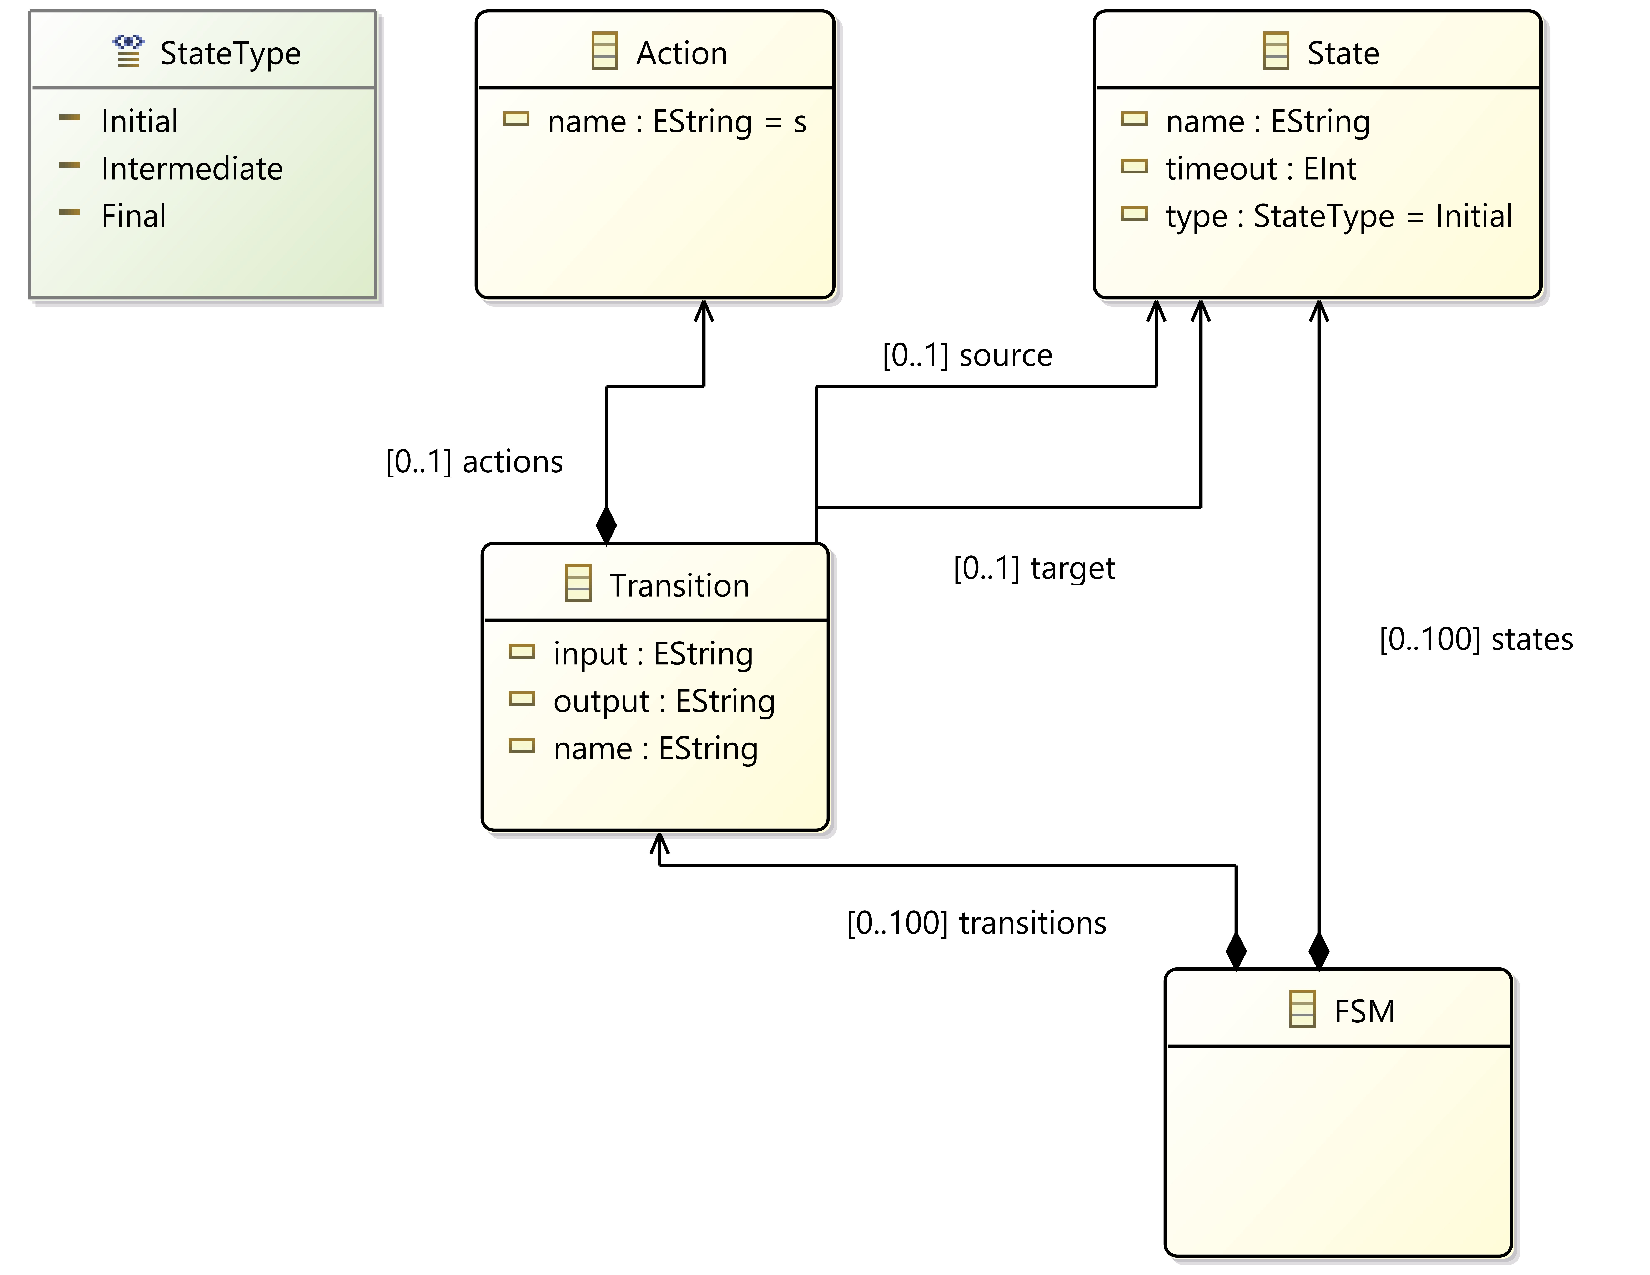
\includegraphics[width=8 cm]{Figures/ecorediagram.pdf}
    \caption{The ecore diagram of a FSM.\label{fig:ecoremodel}}
\end{figure}

\begin{figure}[H]
    \centering
    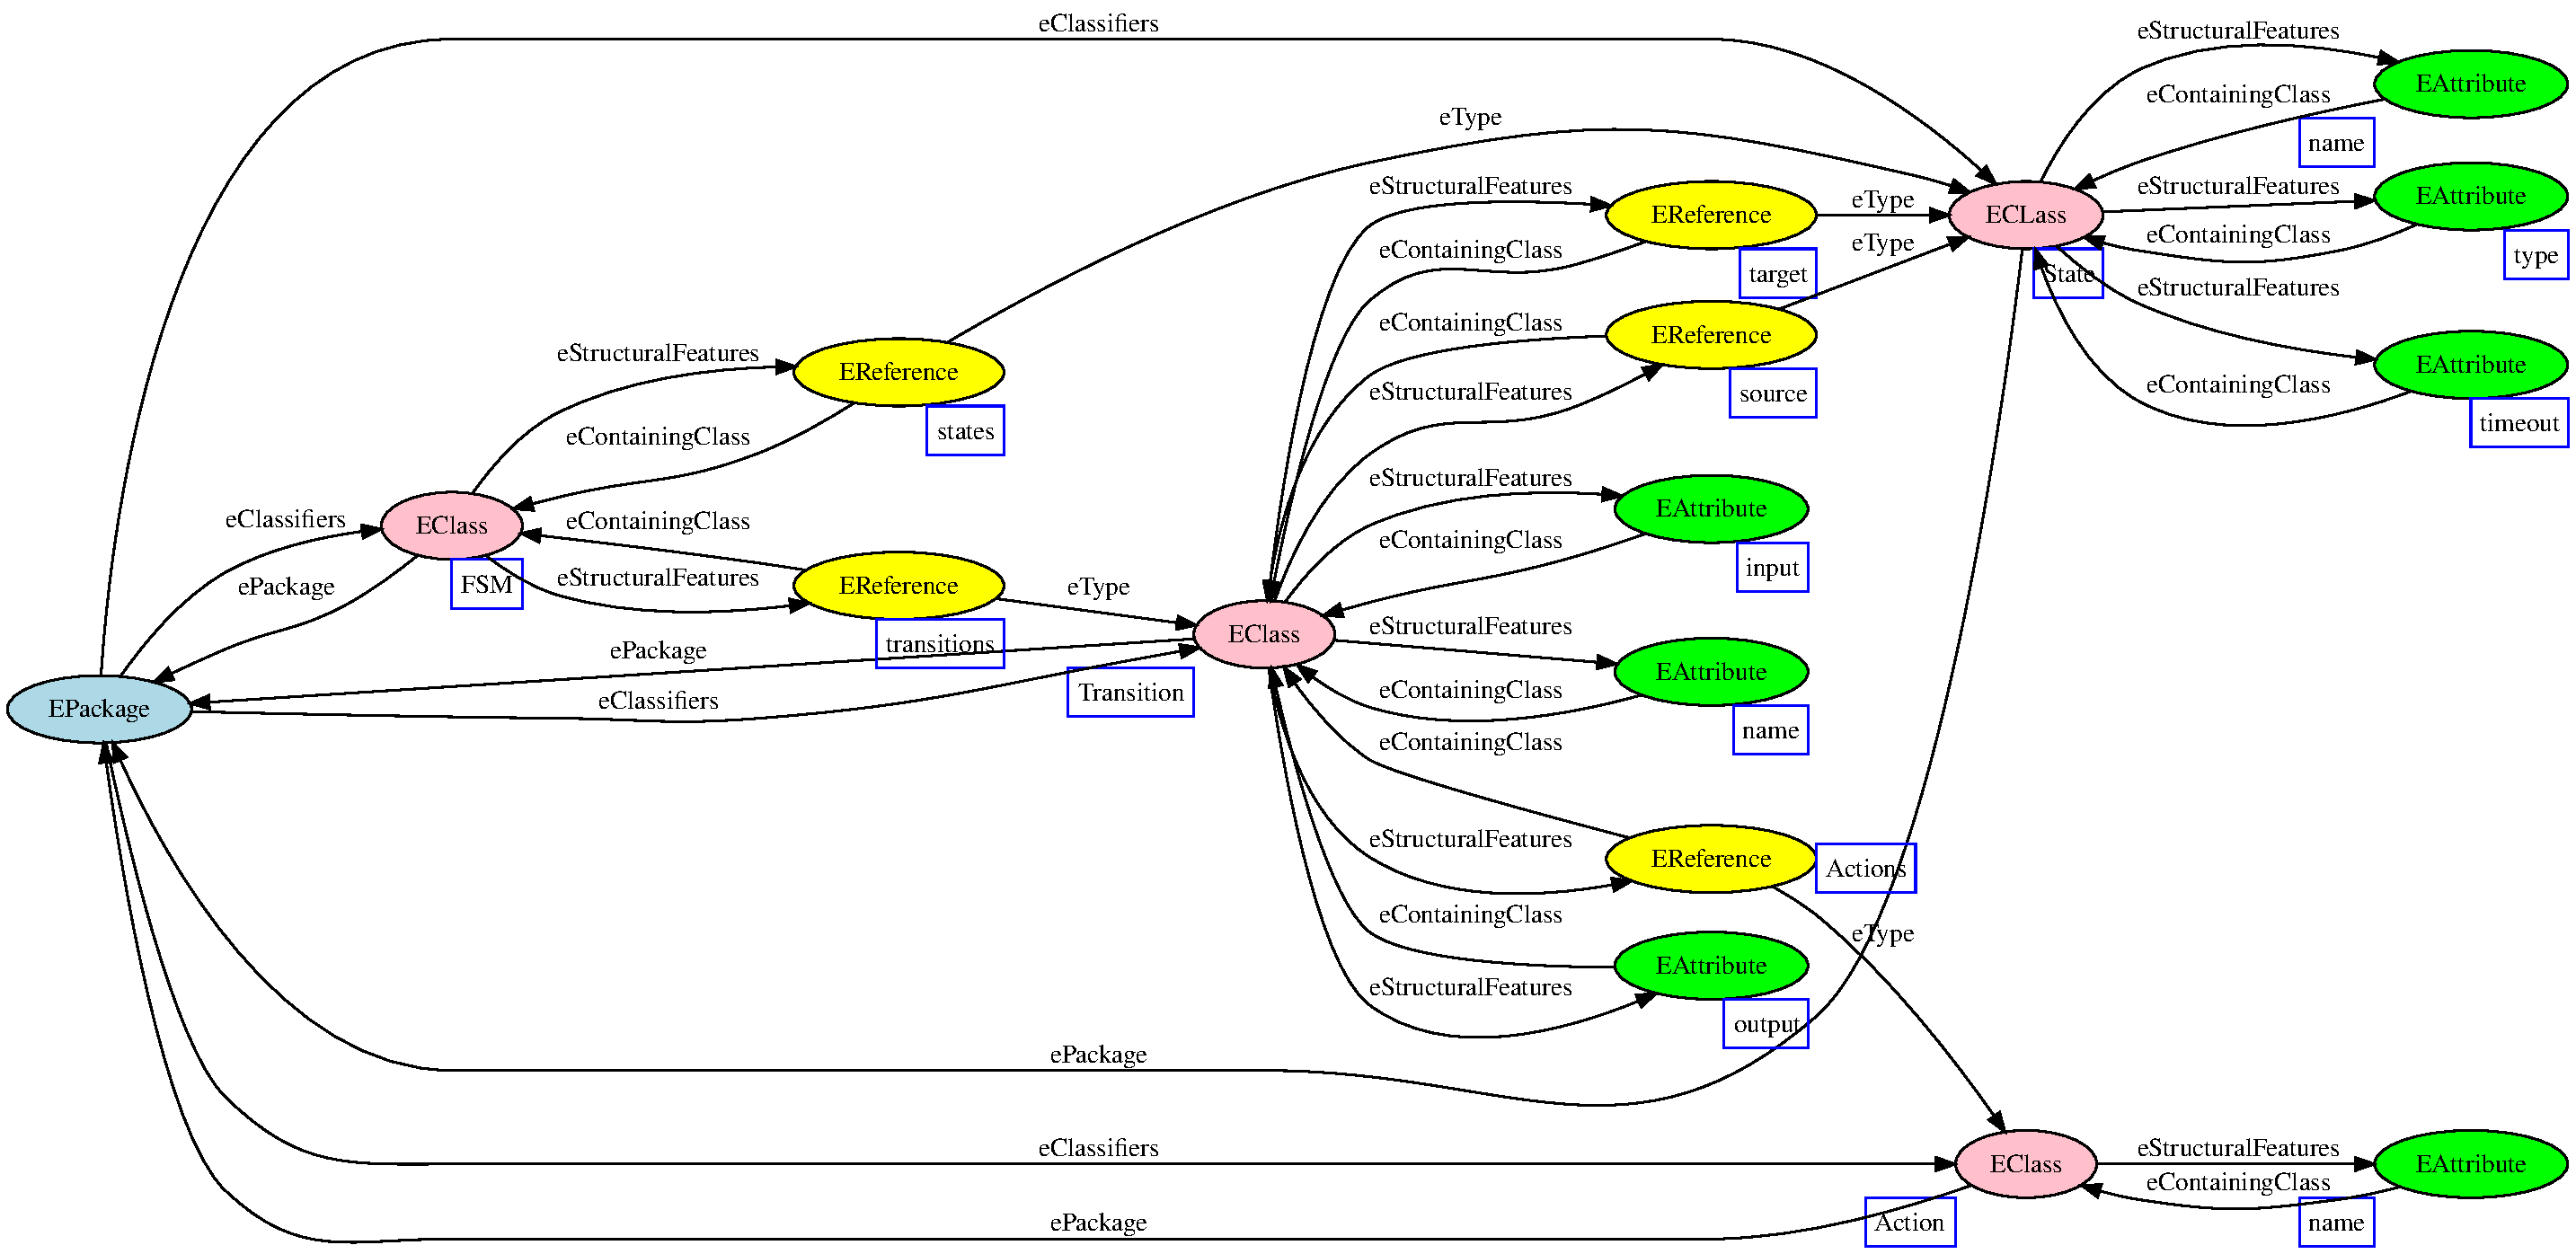
\includegraphics[width=\textwidth]{Figures/ecoregraph.pdf}
    \caption{The corresponding graph of the metamodel in Figure~\ref{fig:ecoremodel}.\label{fig:ecoregraph}}
\end{figure}

\begin{figure}[H]
    \centering
    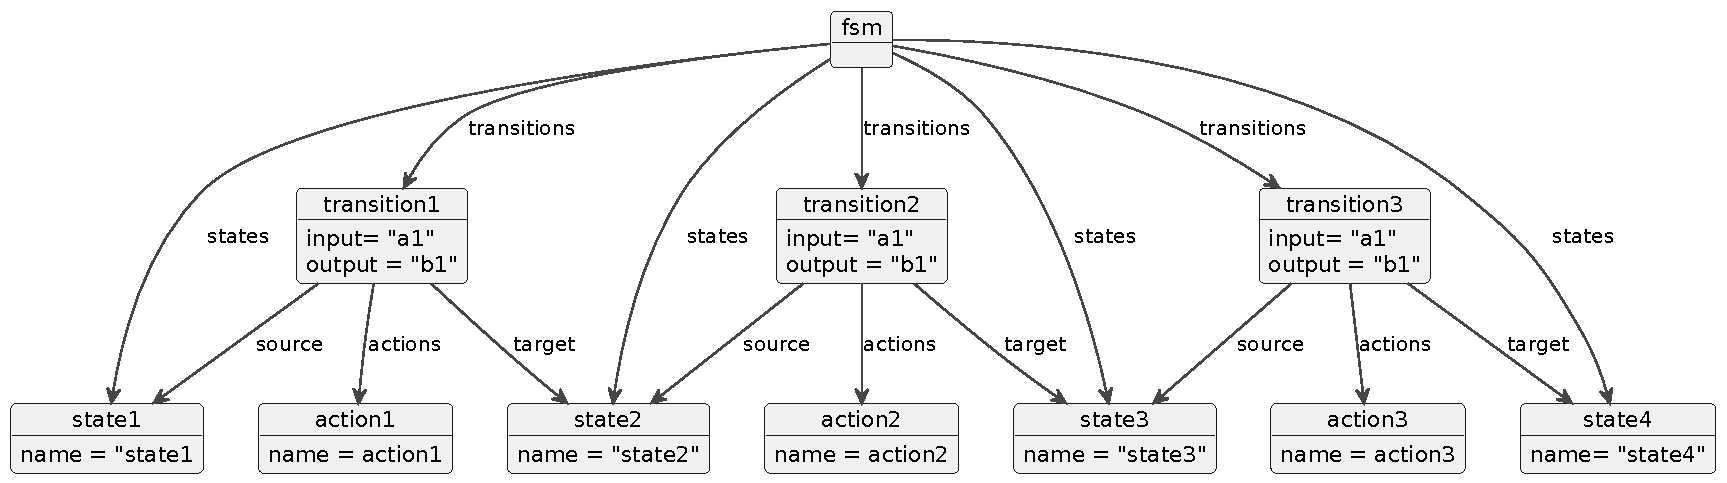
\includegraphics[width=\textwidth]{Figures/object diagram.pdf}
    \caption{An instance model of the FSM in Figure~\ref{fig:ecoremodel}.\label{fig:objectdiagram}}
\end{figure}

\begin{figure}[H]
    \centering
    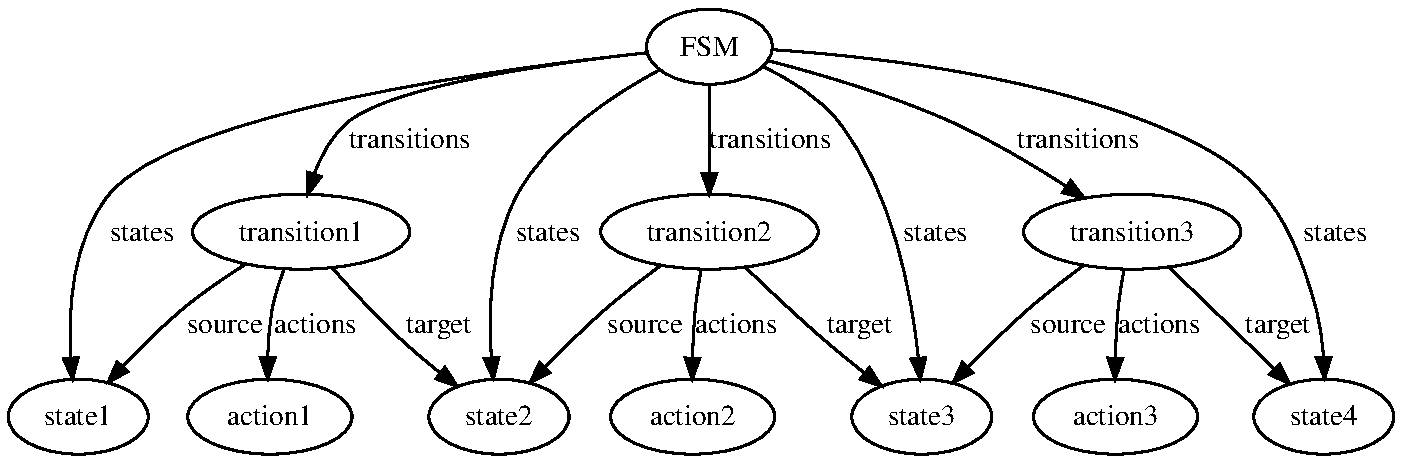
\includegraphics[width=10 cm]{Figures/object graph.pdf}
    \caption{A graph corresponding to the instance model in Figure~\ref{fig:objectdiagram}.\label{fig:objectgraph}}
\end{figure}


\section{Encoding Process} \label{sec:EncodingProcess}
The architecture of our proposed encoding of models is illustrated in Figure~\ref{fig:Structure}. It consists of three main technical spaces: model engineering, data gathering, and graph presentation technical spaces. \rev{In the first phase the current loader reads the models with lxml into an in-memory cache. An earlier loader used PyEcore; that is not the loader timed in Section~\ref{sec:evaluation}.}

In the next phase, the MoEGL configuration is loaded to check for necessary adaptations. \rev{The MoEGL configuration, written by the user, conforms to the class diagram in Figure~\ref{fig:DSL_Diagram}.} It is described in more detail in the next section. \rev{The configuration then selects classes and features from that cache.} The data are organized into three levels including node data, edge data, and attribute type data. For example, the organization of the node and edge data for the model in Figure~\ref{fig:ecoremodel} would be as follows: The node data contains one EPackage file with the EPackage data, four EClass files with the EClass object data, five EReference files with the EReference object data, and seven EAttribute files with the EAttribute objects data. The edge data files contain EPackage--EClass edges, EClass--EPackage edges, EClass--EReference--EClass edges, EClass--EReference edges, and so on.

Finally, the data extracted from the organized files are transformed into an in-memory representation according to the user needs specified in the MoEGL configuration. We provide two output graph formats, including the NetworkX and Heterogeneous PyTorch Geometric (HPyG) graphs. MoEGL is described in more detail in the following section.

Existing works in the literature employ NetworkX for representing models as homogeneous graphs. We add support for mapping models to heterogeneous graphs. These graph types are more precisely aligned with the model structures, by supporting node types associated with sets of attributes, thus allowing object attributes to be directly represented.

\begin{figure}[H]
    \centering
    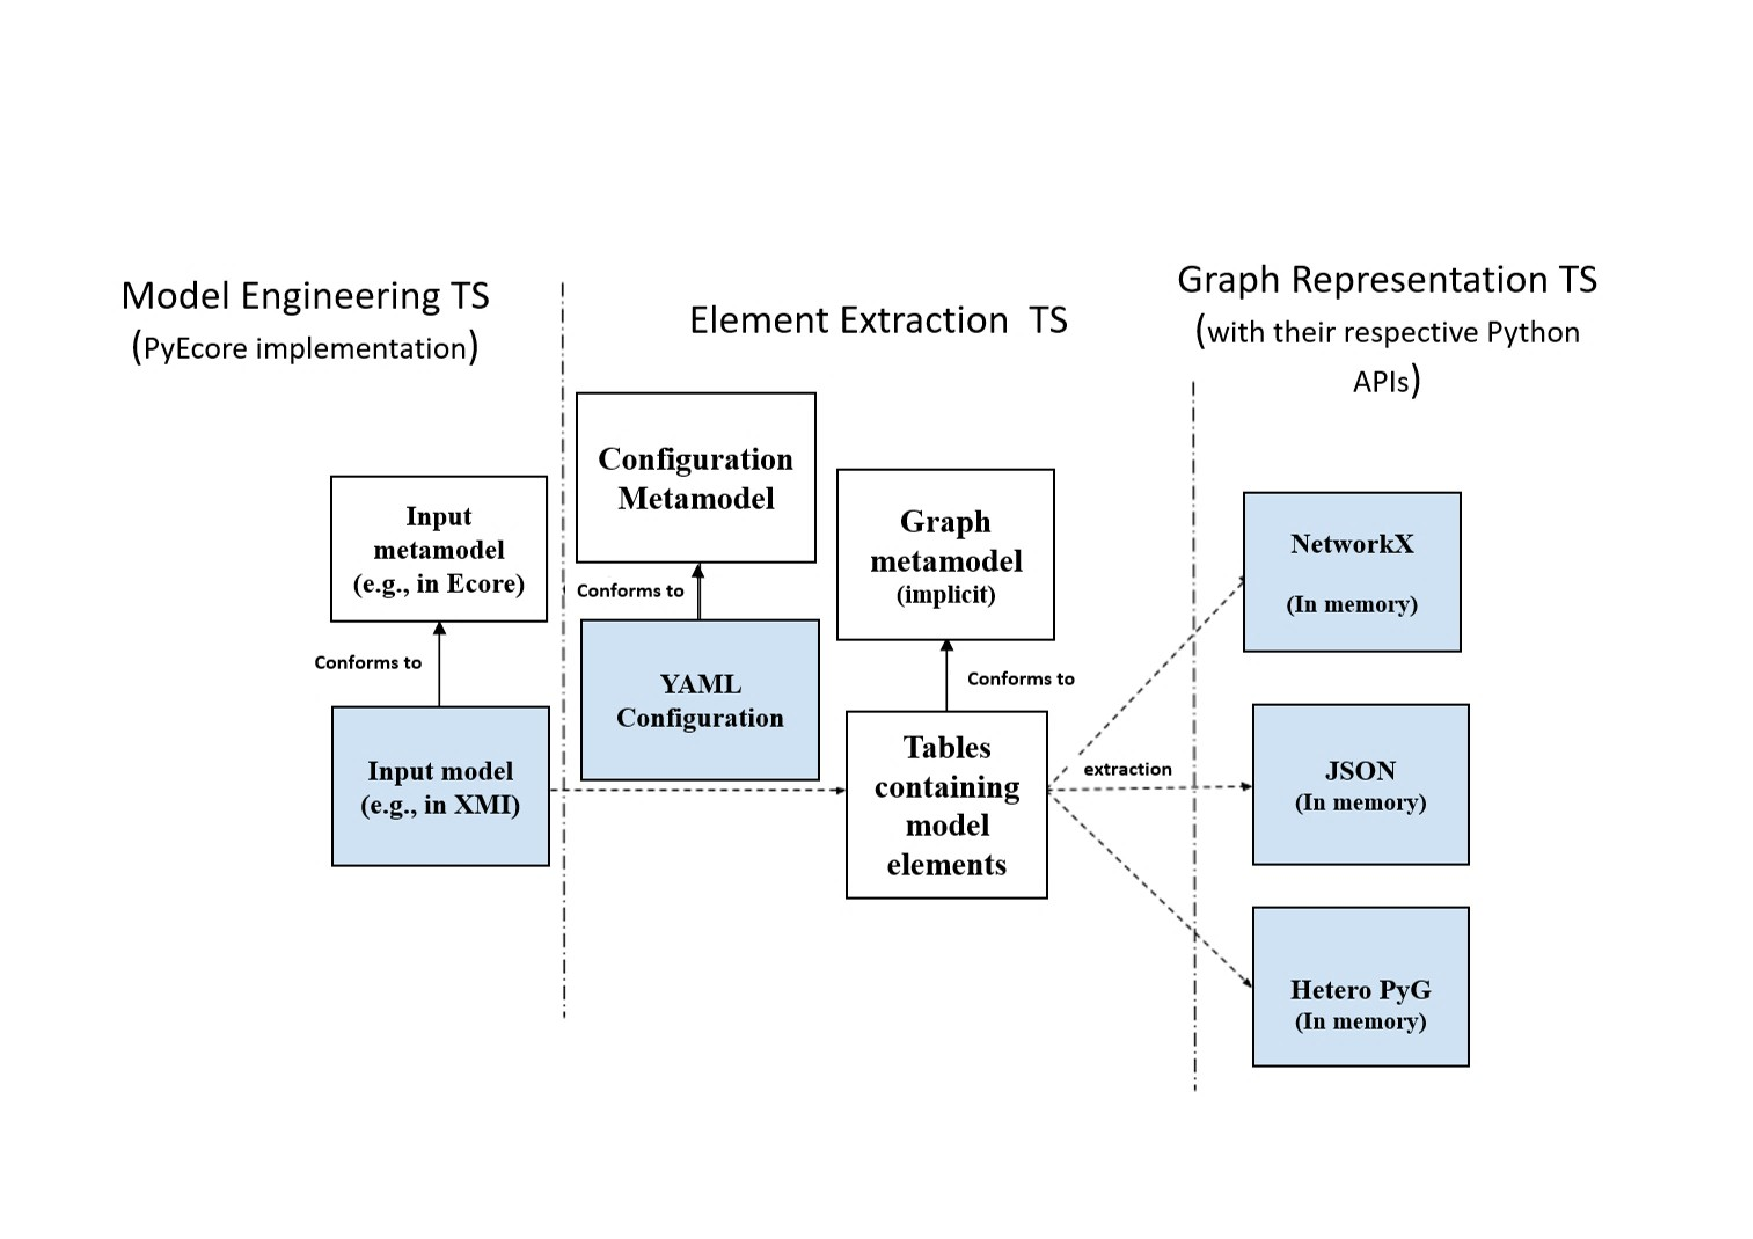
\includegraphics[width=10 cm, trim = 2cm 3cm 2cm 2cm]{Figures/structure.pdf}
    \caption{The architecture of the proposed process.\label{fig:Structure}}
\end{figure}

\subsection{Heterogeneous Graph Construction} \label{Heterogeneous graph}
A heterogeneous graph is a general graph model that can represent multi-typed entities and relations. As defined by Sun et al.~\cite{sun2012mining}, a heterogeneous graph G is represented as \(G = \{V, E, \phi, \psi\} \) where V is the set of nodes, E is the set of edges, \(\phi(v)\) assigns a type to each node $v$, and \(\psi(e)\) assigns a type to each edge $e$. More specifically, \(T_v = \{\phi(v): \forall v \epsilon V\}\) contains the distinct node types defined in the graph schema, and \(T_e = \{\psi(e): \forall e \epsilon E\}\) contains the distinct edge types. This typing of both nodes and edges allows a heterogeneous graph to represent diverse semantic entities and their interconnectivity in a structured manner. The graph degenerates into a regular homogeneous graph when \( \mid T_v \mid = \mid T_e \mid = 1 \), meaning there is only one node and one edge type.

Here, we undertake an in-depth examination of the encoding technique applied to various input models, such as metamodels and instance models, comparing this encoding approach to representations utilized in prior work. Considering the metamodel of the FSM in Figure~\ref{fig:ecoremodel}, it contains 1 node of type ``EPackage'', 4 nodes of type ``EClass'', 5 nodes of type ``EReference'', and 7 nodes of type ``EAttribute''. As illustrated in Figure~\ref{fig:ecoregraph}, nodes sharing an equivalent color within the graph possess an identical type, attribute set, and relationship configuration. When metamodels are encoded as graphs, node attributes serve to represent the properties belonging to each object (referred to as metadata). For instance, an ``EClass'' node might contain an ``abstract'' attribute, whereas an ``EReference'' node could outline attributes such as ``lowerBound'', ``upperBound'', ``ordered'', ``unique'', ``required'', ``changeable'', and ``volatile''. These properties aid tasks involving the architectural structure of metamodels, including but not limited to model generation, completion, and ML applications.

Considering the instance model depicted in Figure~\ref{fig:objectdiagram}, it contains four types of nodes (FSM, Transition, State, and Action) and five types of edges (transitions, states, source, target, and actions). Additionally, the individual nodes themselves carry substantial attribute information (e.g. name, input, output, type, and timeout). Furthermore, the various relationships between the nodes convey richer semantic information. Due to the diversity of node and edge types present, a homogeneous graph alone is unable to represent all facets of the information within the model. When handling nodes and relations with different semantics in such models, graphs originally proposed using homogeneous structures may encounter notable obstacles. In previous work, node types in homogeneous graphs have been managed by defining a ``type'' attribute for each node. HGNNs are able to learn on attributes with different types stored for each node type, effectively handling the inherent complexity of heterogeneous graphs. This complexity arises because, unlike homogeneous graphs where all nodes share the same set of attributes, heterogeneous graphs contain multiple types of nodes and edges, each with unique attributes and relationships. HGNNs address this challenge by utilizing specialized mechanisms to process and integrate these diverse attributes and structural information. They employ tailored aggregation functions to capture the semantic and structural information unique to each node type, ensuring that the rich semantic and structural diversity of heterogeneous graphs is preserved and leveraged effectively for various applications.

\section{MoEGL: Encoding Configuration DSL} \label{Sec:encodingconfigurationDSL}
We propose MoEGL, a DSL to flexibly encode domain models as graphs tailored to users' needs. We defined a list of requirements for MoEGL, that we used to drive its design. We list them here. \rev{Section~\ref{Sec:Experiments} answers the three research questions of Section~\ref{sec:rqs}: fidelity, cost, and the effect on a learner.}

\begin{itemize}
    \item MoEGL syntax must be simple, clear, and unambiguous to avoid any misinterpretations. Static checks on model elements are also important. This includes ensuring the uniqueness of class and feature names within the same package.
    \item The language must be familiar and intuitive for users. Using YAML, a widely known data serialization format, can help with this.
    \item There also needs to be a strategy to prevent naming collisions between generic encoding properties and meta-model elements
    \item All EMF metamodels (including cyclic ones) have a hierarchical containment structure. We want to organize MoEGL based on this structure, which is already familiar to EMF practitioners. This way we can also statically assess consistency with the EMF metamodel, and its coverage. As a consequence of this choice our handling of cycles is limited, as we can copy them or remove them, but we can not create new cycles. This is however sufficient for our needs, since the encoding process does not generally modify the structural properties of the graph.
    \item It is crucial to support different output formats suitable for diverse user needs.
    \item The language must allow access to all meta-model elements and features via YAML sections.
    \item Crucially, MoEGL needs options to flexibly adapt the meta-model structure as required. For example, renaming model elements or encoding attribute values. This level of customization is key to meeting varied user requirements.
\end{itemize}
\rev{These items are the design aims. The evaluation measures how far the language meets them: the reproduced graphs, a configuration of 14 to 29 lines, the running time against the Java encoder, and the classification result. A study with practitioners is future work.}

We implement our language as a schema defined within the YAML format. YAML~\cite{ben2009yaml} serves as a data serialization framework. It incorporates various segments such as structural details and raw informational payloads. YAML presents a relatively straightforward usage while maintaining compatibility with many common programming languages like Python. The relationships, characteristics, and organization of MoEGL are visualized conceptually through the class diagram presented within Figure~\ref{fig:DSL_Diagram}. This diagram outlines the primary abstractions, their attributes, and the connections between these abstractions that underlie the structure and functionality of the language that has been constructed to serve the needs of the targeted domain. The structure of possible sections and values in YAML is shown in Listing~\ref{code:Yaml}. All the code implementations of the proposed DSL are available on GitHub at \url{https://github.com/Z-Rajaei/MoEGL}.

\begin{figure}[H]
    \centering
    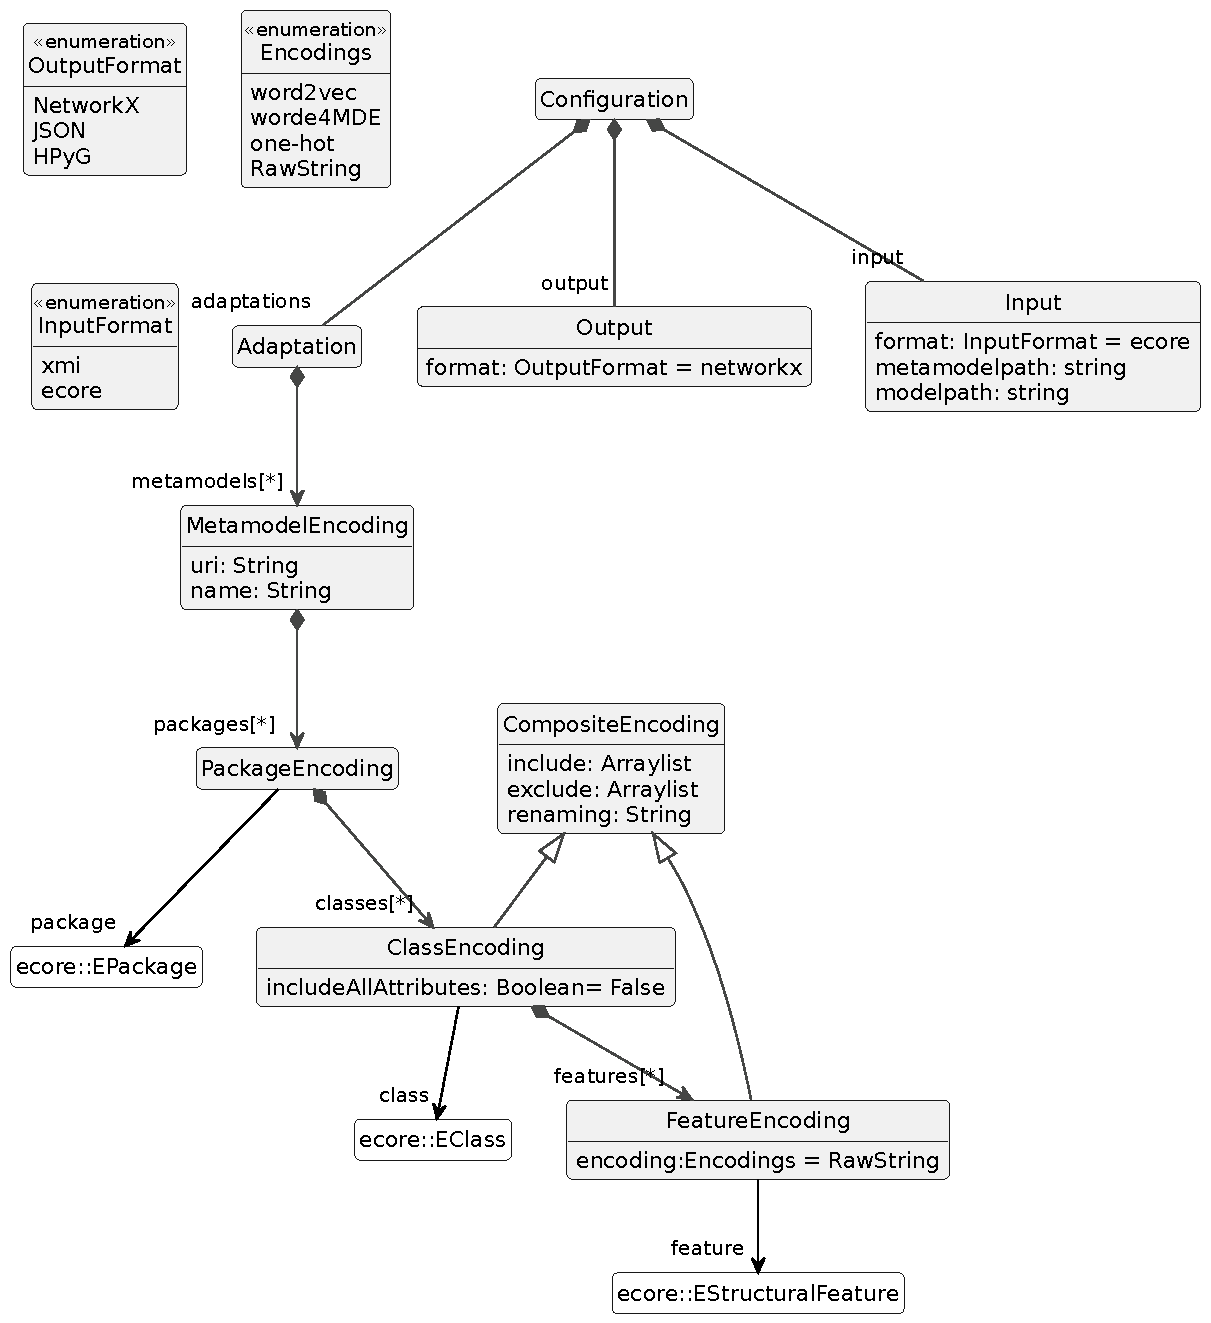
\includegraphics[width=12 cm]{Figures/DSL_diagram.pdf}
    \caption{The class diagram of MoEGL.\label{fig:DSL_Diagram}}
\end{figure}


\begin{program_}[H]
\footnotesize
\begin{verbatim}
input:
  format: "xmi"
  metamodelpath: "examples/running_fsm/fsm.ecore"
  modelspath: "examples/running_fsm/models"
output:
  format: "NetworkX"
adaptations:
  metamodels:
    packages:
      FiniteStateMachine:
        uri:
          www.fsmmetamodel.com:
            classes:
              include: ["FSM", "Transition", "State"]
              exclude: ["Action"]
              includeAllAttributes: false
              FSM:
                include: ["transitions", "states"]
                features:
                  transitions:
                    renaming: "trans"
              Transition:
                include: ["source", "target", "name"]
                features:
                  name:
                    encoding: "RawString"
\end{verbatim}
\caption{\rev{The MoEGL syntax, as a configuration that the tool loads and runs on the running example.}}
\label{code:Yaml}
\end{program_}

\rev{Listing~\ref{code:Yaml} is the syntax of every configuration in this paper. The three top-level keys are \texttt{input}, \texttt{output} and \texttt{adaptations}. \texttt{input.format} is \texttt{ecore} or \texttt{xmi}. \texttt{input.metamodelpath} is the metamodel file and \texttt{input.modelspath} is the directory of models. \texttt{output.format} is \texttt{NetworkX} or \texttt{HPyG}. Each entry of \texttt{adaptations.metamodels.packages} is a package name whose \texttt{uri} selects the package, and the \texttt{classes} object under that URI holds the filters. \texttt{include} and \texttt{exclude} name classes or, inside one class, features. \texttt{includeAllAttributes} is a Boolean. A class is configured under its EClass name: \texttt{renaming} changes that name in the graph, and \texttt{features} names a feature, which may be an attribute or a reference: \texttt{renaming} applies to either, and \texttt{encoding} applies to an attribute value. The encoding is one of \texttt{RawString}, \texttt{word2vec}, \texttt{worde4mde} and \texttt{one-hot}. Paths are relative to the MoEGL package root. Listing~\ref{code:Yaml} and the three YAML listings that follow it were loaded and executed on the files in \texttt{examples/running\_fsm}. The experiment listings are the configurations already used for Tables~\ref{tab:experimentations} and~\ref{tab:evaluation}.}


\rev{The three sections of a configuration are \texttt{input}, \texttt{adaptations} and \texttt{output}, as written in Listing~\ref{code:Yaml}.} The ``adaptations'' section allows for customizing how the elements from the metamodel are encoded as nodes and edges in the graph. This preprocessing is necessary to transform the models into a format that is suitable for various ML tasks. Each adaptation incorporates one or more ``MetamodelEncoding'' components empowering the user to get to the intended metamodel through the ``name'' and ``URI'' addresses of its package. Under each ``PackageEncoding'' are ``Class Encoding'' components that allow the user to selectively include or exclude which model element classes will be represented as nodes in the final encoded graph. Individual classes can then be further configured via their name, where the features of each class can be selectively included or excluded at the attribute and reference level. The user can also specify whether all class attributes participate in encoding using ``includeAllAttributes''. We do not need to provide OCL constraints, since we define a policy to unambiguously handle every combination of these operators. In our policy, attribute exclusions have the highest priority, followed by attribute inclusions. For instance, if ``includeAllAttributes'' is followed by an ``exclude'', the DSL will include all the attributes that are not explicitly excluded.

The capabilities of the MoEGL configuration allow users to selectively determine which model aspects are included or excluded in/from the final representation. Individual characteristics can be included or excluded from the final encoded graph structure by utilizing their given names or labels in conjunction with the ``include'' and ``exclude'' directives. Features can be included or excluded by name using ``include'' and ``exclude''. A feature can be an attribute or a reference. If the excluded feature is a containment reference, the program simply removes the reference and not the target class. Therefore, if we also need to remove the target, it should be excluded explicitly by the ``exclude'' option in the class section. When a containment reference is excluded, the program removes the reference because it represents the relationship or linkage between elements rather than the elements themselves. The target class, being a separate entity, is not automatically removed to preserve the integrity of other potential references or usages within the model. If the target class were to be removed automatically, it could inadvertently affect other parts of the model that rely on it. Therefore, to ensure precise and controlled modifications, the user must explicitly exclude the target class in the class section. This approach maintains the model's consistency and prevents unintentional deletions that could disrupt the overall structure and functionality of the model.

Each class offers attribute configuration. Similarly, the user can access classes as shown in the diagram. Renaming modifies element names for tasks involving the comparison of metamodels with identically named but distinct attributes. For instance, the user can specify in the DSL that a ``surname'' attribute should be renamed to ``lastname'', so that it will share the same encoding of another ``lastname'' attribute in the metamodel.
The feature encoding section specifies how the values of attributes and references should be represented, such as raw strings or using vector representations obtained via techniques like word2vec. Further explanation is provided regarding these encoding representations and techniques later on. The ``input'' meta-schema specifies the data format of source models, as the declarative language is designed to encode models defined in both Ecore and XMI formats. Relevant file paths must also be set for both the metamodel and models. The desired output graph format such as NetworkX or HPyG is then configured within the output section settings. Proper configuration of input data retrieval and desired output formatting is crucial for effectively transforming models into machine-readable graph structures while preserving original semantic meaning.

The declarative schema language therefore provides access and manipulation capabilities applicable to full metamodels, individual model classes, and even single attributes or references. The second major processing stage depicted in Figure~\ref{fig:Structure} relies on these pre-encoding adaptations and configurations by way of a specified Python method to selectively check and include only relevant model aspects.

\subsection{\rev{Semantics of a Configuration}}\label{sec:semantics}
\rev{The list at the start of this section states the design aims. The rules below are the behavior of the loader and of the adaptation step. A configuration does not receive a coverage score.}

\begin{itemize}
    \item \rev{\textbf{Coverage.} With no class \texttt{include} list, every class is kept except those named by \texttt{exclude}. With an \texttt{include} list, a class is kept when its name, or the name of one of its supertypes, appears in that list. \texttt{exclude} is applied first, so a class named in both lists is dropped. A dropped class removes its objects and every edge that touches them. Inside a kept class, \texttt{exclude} is again applied first. If any applicable class section gives an \texttt{include} list, a feature is kept only when its name is in the union of those lists. If no such list is given, every reference is kept, and an attribute is kept only when \texttt{includeAllAttributes} is true. Dropping a feature removes that attribute or that edge. The target object stays until its own class is excluded. A rule written on a supertype applies to its subtypes.}
    \item \rev{\textbf{Conflict resolution.} The two conflicts are a name present in both \texttt{include} and \texttt{exclude}, and two sections that rename the same element. Exclusion wins in the first case, for classes and for features. In the second case the renaming is taken from the most specific class section that defines it: the object's own class before a supertype. Feature renaming uses the same order.}
    \item \rev{\textbf{Identity and cross-resource references.} Each object receives an integer identity in the order the loader creates it. An edge stores those integers. A reference token is resolved inside the same file: a fragment that starts with \texttt{/} walks the containment tree, and any other token is an \texttt{xmi:id} or an attribute marked \texttt{iD}. A token of the form \texttt{uri\#fragment} is kept as an edge inside this file in two cases: the URI names this file, or the fragment still resolves here after the resource was renamed, in which case the URI is recorded in the load cache as repaired. An absolute URI, and a URI that starts with \texttt{platform:} or \texttt{pathmap:}, produces no object and no edge. A relative URI whose file exists beside the model is treated the same way: the external resource is out of scope. A token that contains \texttt{\#} and does not resolve is stored as an attribute whose name is the feature name plus \texttt{Name} (for example \texttt{eTypeName}), holding the name after \texttt{\#}. A root or a child from a foreign namespace is skipped.}
    \item \rev{\textbf{Cycles.} Containment is walked as a tree, in document order, and each containment child receives an edge. A non-containment reference becomes an edge to an object that already exists, so a cycle that the file already contains is copied. Filtering drops an edge by dropping one of its ends or by excluding its feature. The one edge added beyond the serialized references is the opposite named by the metamodel: when a feature records an opposite, and that opposite feature exists on the target class and is not derived, the loader writes the reverse edge under the opposite's name. On the Ecore metamodel used for these experiments, \texttt{EReference.eOpposite} records no opposite, so an \texttt{eOpposite} edge is written only where the file serializes it. No configuration key inserts any further edge.}
    \item \rev{\textbf{Multi-edges.} The NetworkX graph is a \texttt{MultiDiGraph}. The loader stores at most one edge for each triple of source identity, target identity and feature name, so a second value of the same feature toward the same object does not create a second edge. Two features between the same pair remain two edges, distinguished by the edge key \texttt{type}. A multi-valued feature toward distinct objects is one edge per object.}
    \item \rev{\textbf{Edge attributes.} The only key stored on an edge is \texttt{type}, and its value is the reference name, after renaming. The encodings \texttt{RawString}, \texttt{one-hot}, \texttt{word2vec} and \texttt{worde4mde} apply to attribute values on nodes. A feature that is itself named \texttt{type} collides with the NetworkX node key of that name, and that writer raises an error. The heterogeneous writer keeps the class as the node type and stores the value in the feature tensor. Section~\ref{sec:limits} repeats this boundary.}
\end{itemize}

\subsection{Encoding Attribute Values}\label{sec:avalues}
\rev{Numerical attributes are stored as their raw values unless the configuration says otherwise. For a string, the configuration names one of three encoders: a word2vec model fitted on the dataset being encoded, the pretrained WordE4MDE vectors~\cite{lopez2023word}, or a one-hot vector.}

\rev{Names are split before either embedding is applied. Non-alphanumeric characters are separators, and a camelCase or PascalCase boundary is a separator, so \texttt{hasCustomer} becomes the tokens \texttt{has} and \texttt{customer}. Digits stay with the token they are attached to until a separator. The vector of a value is the mean of the vectors of its known tokens.}

\rev{The local word2vec model is a skip-gram Word2Vec fitted once on every token of the dataset (dimension 64, window 3, minimum count 1, 20 epochs, one worker, seed 42). A value with no token, or whose tokens are all absent from that vocabulary, becomes the zero vector. On one small instance the training text is a handful of names, and the coordinates stay near the random initialisation, whose scale is \(0.5/d\). The previous version of this article printed such a vector, with entries around \(\pm 0.01\), from the running example. That vector was not a trained embedding, and we have removed it. A locally fitted model is useful when the dataset is large enough to estimate co-occurrence; the running example is not such a dataset.}

\rev{That fit, and the vocabulary of a one-hot encoding, is built on every model passed to it. When the encoded values are later used as features of a supervised split, the fit has to be called on the training fold alone, and the fitted model is then applied to the validation slice and to the test fold. A token absent from the training vocabulary stays the zero vector. Fitting on the whole corpus before the split would place test names inside the vectors. Encoding a dataset that has no held-out split, such as the timed re-encoding in Section~\ref{sec:evaluation}, uses the same fit on the whole set.}

\rev{WordE4MDE is a skip-gram model trained by its authors on a large corpus of element names from real models (300 dimensions)~\cite{lopez2023word}. MoEGL loads those vectors and applies the same tokeniser. A name whose tokens are all unknown becomes the zero vector. In the classification experiment of Section~\ref{sec:learning}, a linear SVM on the mean WordE4MDE vector of each model scores \(0.808\pm0.024\) balanced accuracy, level with the TF-IDF baseline on element names, and a GIN that uses the same vectors as node features scores \(0.770\pm0.029\). We therefore provide WordE4MDE for datasets too small to fit word2vec. On this classification task it matches the bag-of-names baseline.}

Categorical attributes that describe element or relationship types can be encoded using one-hot encoding. This involves mapping each unique category to a binary vector, with a 1 in the index of the present category and 0s elsewhere. One-hot encoding transforms categorical data into a numerical format while retaining the distinction between different categories. This encoding supports various predictive tasks involving element types.

We were also able to implement one-hot encoding for the same reason, as we have the list of possible values for each attribute. This method also provides an additional benefit, allowing the user to parse and run the models once, performing any desired type of encoding or customization on the models multiple times.
Figure~\ref{fig:fusion} illustrates the described process. The structure and attributes of each model are derived and extracted from the models. The final graph contains both the relational framework of the associations between models as well as the numerically encoded attribute values appointed to each individual node. Once completed, the graphs are then input as data into a GNN system. The neural network will utilize the combined structural and characteristic information from the graph to discern relationships and perform some analytical task, such as classification or prediction, based on the features and connections within the graphical portrayal of the original collection of models.

\begin{figure}[H]
    \centering
    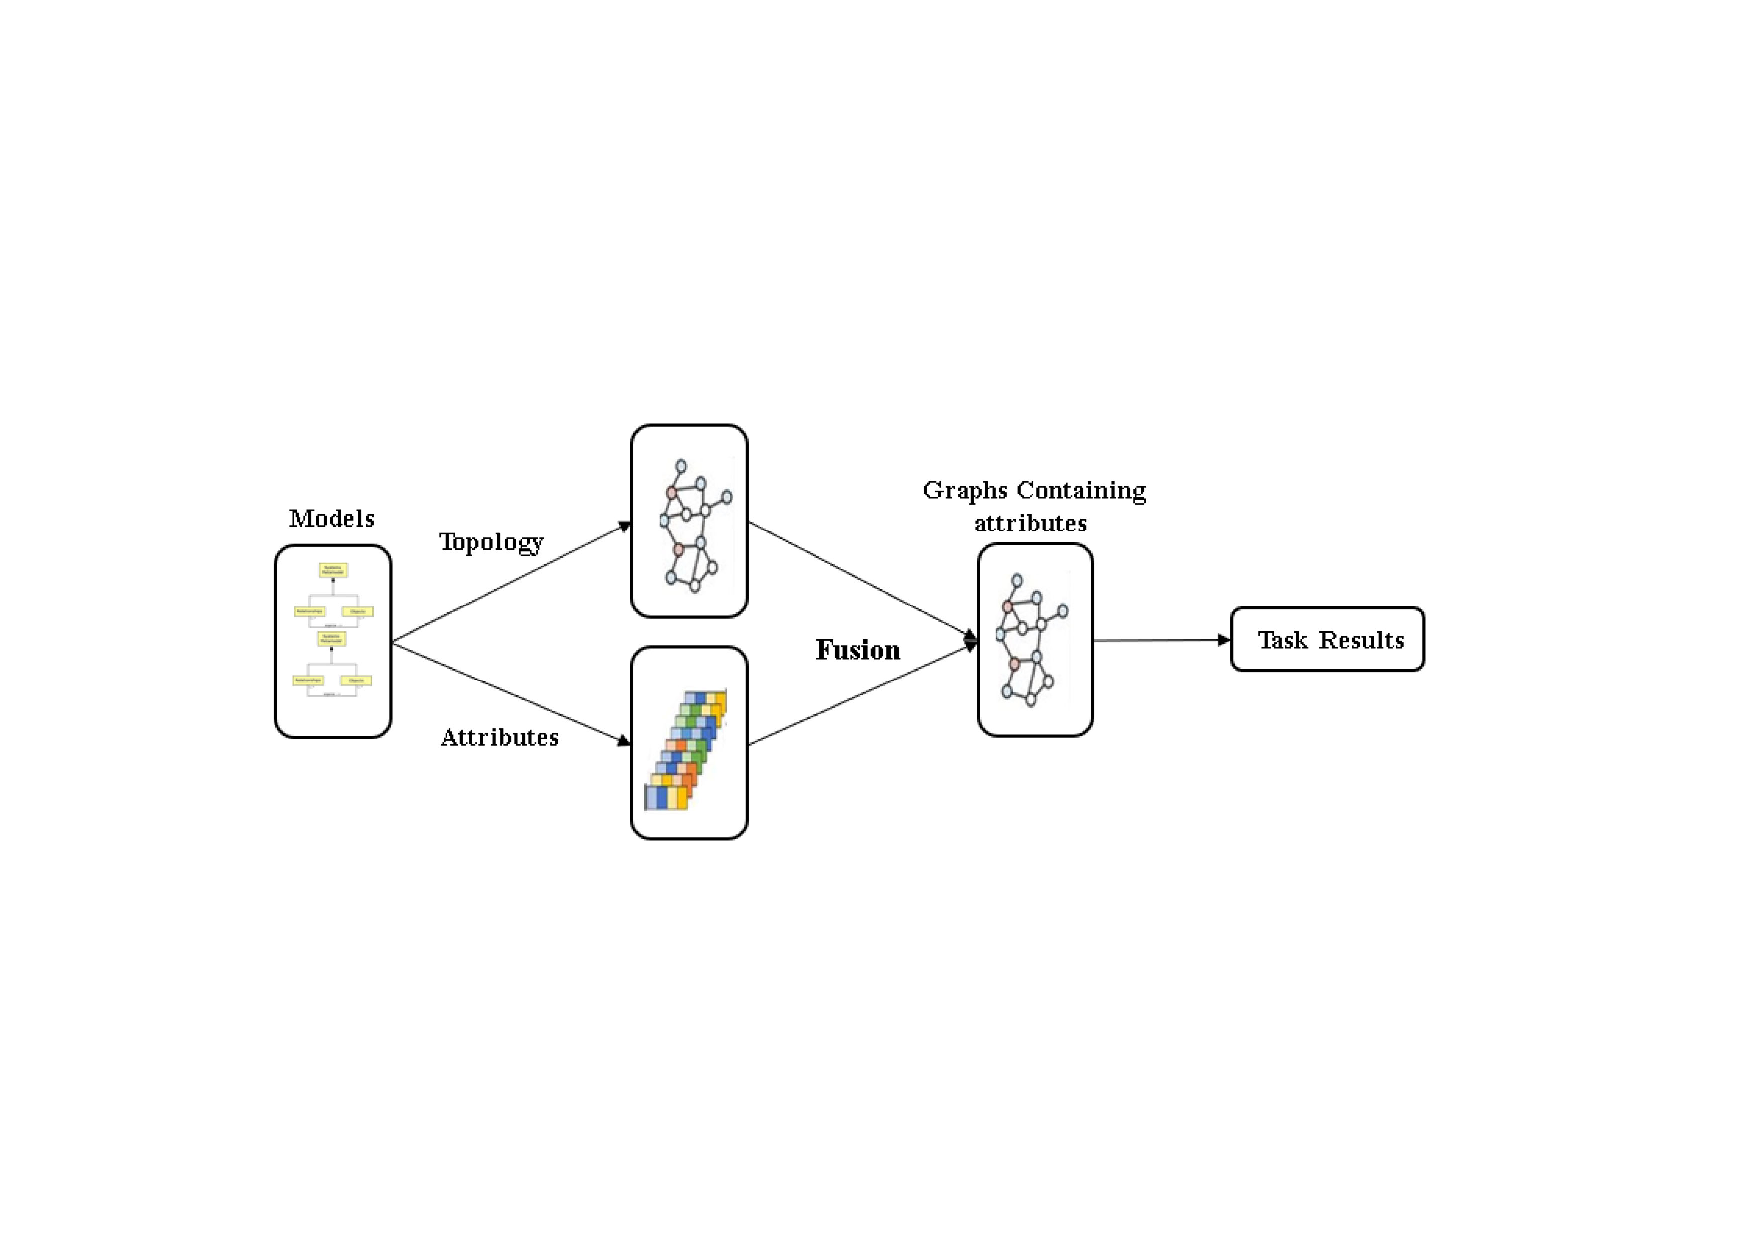
\includegraphics[width=10 cm, trim = 5cm 6cm 6cm 6cm]{Figures/Fusion.pdf}
    \caption{Diagram of extracting model structure and attributes for final graph.\label{fig:fusion}}
\end{figure}

\subsection{Technical Implementation of MoEGL}
In this section, we describe the detailed implementation process of MoEGL, highlighting the key steps involved in transforming models into graph structures suitable for Graph Neural Networks (GNNs). Our approach follows a structured process that includes model traversal, application of filtering rules, \rev{encoding of attribute values on the nodes}, and the construction of both homogeneous and heterogeneous graphs.

\textbf{1. Model Traversal and Element Extraction.}
The first step in our pipeline is the traversal of the input models, which can be provided in either ecore or xmi formats. Depending on the format, we load and traverse the models to extract key elements, such as nodes and edges. During this traversal, the model elements are systematically processed, and for each element, we capture its attributes and references. This hierarchical traversal ensures that all relevant model elements are visited and prepared for inclusion in the resulting graph structure.

\textbf{2. Node and Edge Creation.}
As the model elements are traversed, we generate nodes and edges corresponding to each element and its relationships. Nodes are created for each class instance in the model, with their attributes stored for later use in encoding. Similarly, edges are generated to represent the relationships between different nodes, reflecting the references in the original model. This process ensures that the structure of the input model is accurately preserved in the graph, maintaining the hierarchical and referential integrity of the data.

\textbf{3. Application of Filtering Rules.}
To provide flexibility in model-to-graph transformation, we apply user-defined filters from the configuration file during the graph construction process. These filters allow users to specify which classes and attributes should be included or excluded from the final graph. The filtering is performed in two stages:

Node Filtering: Nodes are included or excluded based on the classes they represent, as defined in the filters. Users can also specify whether all or only certain attributes of a class should be included.
Edge Filtering: Edges connecting nodes are filtered similarly, ensuring that only the relationships of interest are represented in the final graph.
This customizable filtering mechanism allows users to tailor the graph representation to their specific needs, reducing complexity and focusing on the most relevant parts of the model.

\textbf{4. Feature Encoding.}
Once the nodes and edges are filtered, we proceed with encoding their attributes into formats suitable for machine learning. Depending on the user's configuration, various encoding techniques are applied, including:

One-Hot Encoding: Categorical attributes are encoded using one-hot vectors, which is useful for representing discrete variables.
Word2Vec Encoding: For textual attributes, we employ Word2Vec embeddings to capture semantic relationships between words in the model. This provides a dense, continuous representation of text data.
Custom Embeddings (worde4mde): For domain-specific terms in the model, we use a custom embedding technique that maps specific terms to pre-trained embeddings, ensuring that the domain knowledge is accurately reflected in the graph's features.
\rev{These encoding techniques transform attribute values stored on nodes into feature vectors that a GNN can read. An edge keeps the reference name as its type and does not receive one of these vectors. Section~\ref{sec:limits} states this limit together with the others.}

\textbf{5. Graph Construction.}
After encoding the node and edge features, the graph is constructed. We support two types of graph structures:

Homogeneous Graphs: In this configuration, all nodes and edges are of the same type, which is useful for simpler models where there is no need to distinguish between different types of entities.
Heterogeneous Graphs: For more complex models, we construct heterogeneous graphs, where nodes and edges can have multiple types. This allows us to preserve the distinct types of entities and relationships present in the model. The heterogeneous graphs are constructed using libraries such as PyTorch Geometric, which provides efficient handling of different node and edge types for machine learning tasks.

\textbf{6. Output Formats.}
Finally, the constructed graphs can be output in various formats, depending on the user's requirements. We support both NetworkX (for homogeneous graphs) and PyTorch Geometric (for heterogeneous graphs). This flexibility allows the encoded graphs to be used directly in different GNN frameworks, enabling seamless integration with downstream machine learning pipelines.
\rev{The two writers emit an in-memory NetworkX graph and a PyTorch Geometric heterogeneous graph. CSV export, and reconstruction of a graph from CSV, are outside the tool. The tool also does not write the Deep Graph Library~\cite{wang2019deep}, a PyTorch Geometric \texttt{InMemoryDataset}, or Parquet. The time and peak memory in Section~\ref{sec:evaluation} are for the NetworkX encoding of the 500 Ecore models. Scalability past that set is stated there as unmeasured.}


\subsection{Applying MoEGL to the Running Case}\label{sec:applying}
Assume that a user is working with a dataset containing thousands of FSM metamodel instances like the one shown in Figure~\ref{fig:objectdiagram}. He wants to map all these models to NetworkX graphs for use in a ML task. However, there are a couple of constraints he wants to apply: 1) Exclude the ``action'' objects from the models, as they are not relevant to the particular learning task he intends. 2) Rename the ``transitions'' edges to simply ``trans'' for consistency.
The user defines the desired constraints and transformations in a YAML configuration file. As shown in Listing~\ref{code:YamlFSM}, only a few lines of code are needed to exclude the action objects and rename the transition edges.
The adjacency matrix of the instance model in Figure~\ref{fig:objectgraph} generated by applying the encoding of Listing~\ref{code:YamlFSM} is shown in Matrix~\ref{mat:matrix}.
\rev{The eight rows are the objects that remain after the listing drops every Action, in document order: the FSM, transition1, transition2, transition3, state1, state2, state3 and state4. A 1 means a directed reference from the row object to the column object; the matrix does not record the reference name. The first row is the FSM's three transition edges and four state edges. The diagonal entry of that row is 0. The FSM class in Figure~\ref{fig:ecoremodel} has no reference to itself, and the object diagram has no such link. The previous version of this matrix had a 1 in that cell. Running Listing~\ref{code:YamlFSM} on the instance file produces the matrix printed here, with 8 nodes, 13 edges and no self-loop.}
Now the user can run the learning tasks, and modify the YAML file to easily experiment with different preprocessing configurations, applying multiple ``passes'' over the dataset to determine the optimal representation for their ML task.

\begin{mat}[H]
\begin{equation}
    \begin{bmatrix}
0 & 1 & 1 & 1 & 1 & 1 & 1 & 1 \\
0 & 0 & 0 & 0 & 1 & 1 & 0 & 0 \\
0 & 0 & 0 & 0 & 0 & 1 & 1 & 0 \\
0 & 0 & 0 & 0 & 0 & 0 & 1 & 1 \\
0 & 0 & 0 & 0 & 0 & 0 & 0 & 0 \\
0 & 0 & 0 & 0 & 0 & 0 & 0 & 0 \\
0 & 0 & 0 & 0 & 0 & 0 & 0 & 0 \\
0 & 0 & 0 & 0 & 0 & 0 & 0 & 0
    \end{bmatrix}
\end{equation}
\caption{\rev{Adjacency matrix produced by running Listing~\ref{code:YamlFSM}. The diagonal is 0: the FSM object has no edge to itself.}}
\label{mat:matrix}
\end{mat}


\begin{program_}[H]
\footnotesize
\begin{verbatim}
input:
  format: "xmi"
  metamodelpath: "examples/running_fsm/fsm.ecore"
  modelspath: "examples/running_fsm/models"
output:
  format: "NetworkX"
adaptations:
  metamodels:
    packages:
      FiniteStateMachine:
        uri:
          www.fsmmetamodel.com:
            classes:
              exclude: ["Action"]
              includeAllAttributes: false
              FSM:
                features:
                  transitions:
                    renaming: "trans"
\end{verbatim}
\caption{\rev{The configuration that produces Matrix~\ref{mat:matrix}. The class key is the EClass name \texttt{FSM}.}}
\label{code:YamlFSM}
\end{program_}

Let us examine in greater detail the process of configuring a more complex MoEGL program to encode the instance model. The user intends to encode the instance model in Figure~\ref{fig:objectdiagram}, which includes various attributes of different types that must be appropriately encoded. The final goal is to train a neural network to automatically generate similar FSM models. Therefore, representing the attribute values accurately will be crucial to the network's ability to learn.

The user has defined a MoEGL configuration to specify how each attribute should be encoded based on its data type. As shown in Listing~\ref{code:YamlFSMattributes}, the MoEGL configuration outlines that string attributes will use word2vec embeddings to vectorize their values. \rev{On this running example the local word2vec fit has too little text to leave its initialisation, as explained in Section~\ref{sec:avalues}; the printed graph below therefore omits the coordinate dump.} Meanwhile, the type attribute that can take on one of just three class labels will employ a one-hot encoding scheme. This involves transforming each class into a binary vector, with a 1 at the index of the class and 0s elsewhere.

Since the nodes of different types have different attributes and references, the graph representing the instance model must support heterogeneous node and edge types. For this purpose, the user has selected the HPyG library, which provides the necessary functionality. With attributes encoded via the prescribed methods, the graph will contain the rich information needed for the neural network to learn patterns. While NetworkX allows nodes and edges to have different attributes, it does not natively support multiple node and edge types as distinct entities. For this purpose, the user has selected the HPyG library, which provides the necessary functionality to handle heterogeneous node and edge types more effectively.


\rev{As a demonstration, Listing~\ref{fig:outputFSM} is the heterogeneous graph produced by that configuration, not a separate figure and not a matrix.} By examining this data, we can observe details like there being one FSM node, four State nodes, three Transition nodes, and three Action nodes in the graph. The various edge types connecting these nodes are also enumerated. Together, the encoded attributes and graph structure capture the key structural and semantic elements of the instance model for the neural network to analyze and potentially generate new similar FSM models.

\begin{program_}[H]
\footnotesize

\begin{verbatim}
input:
  format: "xmi"
  metamodelpath: "examples/running_fsm/fsm.ecore"
  modelspath: "examples/running_fsm/models"
output:
  format: "HPyG"
adaptations:
  metamodels:
    packages:
      FiniteStateMachine:
        uri:
          www.fsmmetamodel.com:
            classes:
              includeAllAttributes: true
              Transition:
                features:
                  name:
                    encoding: "word2vec"
                  input:
                    encoding: "word2vec"
                  output:
                    encoding: "word2vec"
              State:
                features:
                  name:
                    encoding: "word2vec"
                  type:
                    encoding: "one-hot"
              Action:
                features:
                  name:
                    encoding: "word2vec"
\end{verbatim}
\caption{\rev{Attribute encoding for the running example. The class is \texttt{Transition}, and every \texttt{encoding} key has its colon.}}
\label{code:YamlFSMattributes}
\end{program_}


\begin{program_}[H]
\footnotesize
\begin{verbatim}
HeteroData(
  FSM={ x=[1, 1] },
  Transition={ x=[3, 192] },
  Action={ x=[3, 64] },
  State={ x=[4, 69] },
  (FSM, transitions, Transition)={ edge_index=[2, 3] },
  (Transition, actions, Action)={ edge_index=[2, 3] },
  (FSM, states, State)={ edge_index=[2, 4] },
  (Transition, source, State)={ edge_index=[2, 3] },
  (Transition, target, State)={ edge_index=[2, 3] }
)
\end{verbatim}
\caption{\rev{The heterogeneous graph produced by running Listing~\ref{code:YamlFSMattributes}. Each \texttt{x} shape is (number of nodes, feature width). The State width 69 is a 64-dimensional name vector, the raw timeout and a 4-dimensional one-hot. For state1, \texttt{type=Initial} encodes as $[0, 1, 0, 0]$ (vocabulary Final, Initial, Intermediate, plus an unknown bin) and timeout is the raw value 1. The name coordinates stay at the untrained initialisation of Section~\ref{sec:avalues} and are not printed.}}
\label{fig:outputFSM}
\end{program_}

\rev{Listing~\ref{fig:outputFSM} stores each relation as \texttt{edge\_index} only, under the triple of source type, reference name and target type. That triple is the schema the writer emits. A meta-path is not constructed, and neither is a model that consumes one, such as HAN or MAGNN. Multiplicity and the containment flag stay on the node that declares the reference, when that object is kept in the graph. The HeteroData writer does not emit an edge-feature tensor. Section~\ref{sec:limits} states the same boundary.}



\begin{program_}[H]
\footnotesize
\begin{verbatim}
input:
  format: "ecore"
  metamodelpath: ""
  modelspath: "examples/running_fsm"
output:
  format: "HPyG"
adaptations:
  metamodels:
    packages:
      ecore:
        uri:
          http://www.eclipse.org/emf/2002/Ecore:
            classes:
              includeAllAttributes: false
              EClass:
                include: ["name", "abstract", "eStructuralFeatures"]
                features:
                  name:
                    encoding: "word2vec"
                  abstract:
                    encoding: "one-hot"
              EAttribute:
                include: ["name", "eContainingClass"]
                features:
                  name:
                    encoding: "word2vec"
\end{verbatim}
\caption{\rev{A configuration that encodes the running-example metamodel. \texttt{eType} is a reference, so it stays an edge; the encoding keys apply to the attributes \texttt{name} and \texttt{abstract}.}}
\label{code:yamlecoreAttribute}
\end{program_}



We chose to represent our domain models using objects rather than arrays for improved conciseness and efficiency.
For example, when an array stores objects, each element requires the same name property (e.g. ``FiniteStateMachine'') to be repeated. During deserialization, this would necessitate mapping elements to infer relationships. In contrast, using an object allows each element to be uniquely referenced by name. This is particularly useful for our case where each model element encountered must be matched to determine what it corresponds to in the package and look up details. Listing~\ref{code:YamlFSM} demonstrates this approach, with the ``packages'' property containing an object with a ``FiniteStateMachine'' property. This in turn stores an object with ``uri'' and ``classes'' properties. Notably, ``classes'' is also an object rather than an array, with a property for each EClass name (\rev{\texttt{FSM} in Listing~\ref{code:YamlFSM}}). Importantly, representing the model as an object graph eliminates potential naming collisions. Since the meta-model element names serve as the object keys, and these are guaranteed to be unique, there is no ambiguity in referencing elements during parsing or transformation. Overall, using objects allows our domain models to be encoded more concisely while enabling efficient lookup and disambiguation of elements during the serialization and deserialization process. The object structure directly reflects relationships in the domain model.

\section{Experimentation} \label{Sec:Experiments}

In this evaluation, we aim to demonstrate the expressiveness and usefulness of MoEGL for the model-encoding needs of the MDE community.
To do so, we replicate several encoder implementations from the existing literature on applications of GNNs to MDE. By concisely specifying the mapping configurations in MoEGL, we can perform all the necessary model parsing, element matching, property extraction, and graph construction steps automatically. In this section, each test case will be inspected separately in a dedicated subsection, where the graphs for each one will be recreated using MoEGL.

\subsection{Experiment 1}
First, we validate MoEGL by replicating the experiments by Lopez et al.~\cite{lopez2022generating}. In~\cite{lopez2022generating}, the authors train deep autoregressive models to generate realistic Ecore models. They use four datasets of real models: Ecore-GitHub, Yakindu-GitHub, Rds-GenMyModel, and Yakindu-Exercise.
\rev{We use the Ecore-GitHub dataset, i.e., the 500 real Ecore metamodels released in the replication package of Lopez et al.\ (TCRMG-GNN, release 1.0.0), together with the 500 graphs that their Java encoder produced from these models and that are published in the same package. Their encoder keeps as nodes the objects of type \texttt{EPackage}, \texttt{EClassifier} (\texttt{EClass}, \texttt{EDataType}, \texttt{EEnum}), \texttt{EStructuralFeature} (\texttt{EAttribute}, \texttt{EReference}) and \texttt{EEnumLiteral}, drops annotations, operations, parameters and generic types, keeps nine references as typed edges (\texttt{eClassifiers}, \texttt{ePackage}, \texttt{eStructuralFeatures}, \texttt{eContainingClass}, \texttt{eType}, \texttt{eOpposite}, \texttt{eSuperTypes}, \texttt{eLiterals}, \texttt{eEnum}) and encodes no attribute values. Listing~\ref{code:yamlyakindu} is the complete MoEGL configuration that expresses this encoding. Class-level rules are subtype-aware, so listing \texttt{EClassifier} includes classes, data types and enumerations, and a rule written for \texttt{EStructuralFeature} applies to attributes and references.}

\rev{MoEGL encodes the models into NetworkX multigraphs. Fidelity is certified by a node bijection that preserves every typed edge, obtained by colour refinement and checked edge by edge. This is not NetworkX's default \texttt{is\_isomorphic}, which compares only the shape of the graph and ignores node and edge attributes. Colour refinement starts from the node type, and the bijection is kept only when every typed edge is preserved. On the graphs published by Lopez et al.\ the certificate succeeds for all 500 Ecore graphs, all 500 RDS graphs and all 369 Yakindu graphs. The Yakindu directory contains 377 files; eight have no published graph, so they are not counted as failures. An earlier loader based on PyEcore matched 495 of the 500 Ecore graphs under NetworkX isomorphism. The running time in Section~\ref{sec:evaluation} is for the current loader. The five misses were loader bugs, not DSL bugs: EMF derives \texttt{eType} through the bounds of generic type parameters, which that loader did not implement (three models), and it set \texttt{eOpposite} symmetrically when a model declares it on one side only (two models). Re-running the authors' own Java encoder on the released Ecore files reproduces 492 of 500, because eight released files reference themselves under their original name. The current loader repairs those self-references. All comparison scripts are in the replication package.}


\begin{program_}[H]
\footnotesize
\begin{verbatim}
input:
  format: "ecore"
  metamodelpath: ""
  modelspath: "realModels/Ecore"
output:
  format: "NetworkX"
adaptations:
  metamodels:
    packages:
      ecore:
        uri:
          http://www.eclipse.org/emf/2002/Ecore:
            classes:
              include: ["EClassifier", "EStructuralFeature",
                        "EPackage", "EEnumLiteral"]
              includeAllAttributes: false
              EPackage:
                include: ["eClassifiers"]
              EClassifier:
                include: ["ePackage"]
              EClass:
                include: ["ePackage", "eStructuralFeatures",
                          "eSuperTypes"]
              EEnum:
                include: ["ePackage", "eLiterals"]
              EEnumLiteral:
                include: ["eEnum"]
              EStructuralFeature:
                include: ["eContainingClass", "eType"]
              EReference:
                include: ["eContainingClass", "eType",
                          "eOpposite"]
\end{verbatim}
\caption{\rev{The complete MoEGL configuration that replicates the Ecore encoder of Lopez et al.~\cite{lopez2022generating} (29 lines of YAML).}}
\label{code:yamlyakindu}
\end{program_}

\subsection{Experiment 2}
Rahimi et al.~\cite{rahimi2023towards} presented an interesting approach for generating structurally realistic models using GANs in the context of MDE. The lack of freely available industrial models has motivated the development of model generation techniques. However, realism is often overlooked. Rahimi et al. applied GANs to create new models that closely resemble real ones. A tool is built based on the Eclipse Modeling Framework (EMF) and evaluates the generated models using graph-based metrics. Promising results showed the GAN could produce realistic instances. For validation, they used a dataset derived from a simplified Car Wash Management metamodel in Figure~\ref{fig:ecorecarwash} containing five metaclasses (CarWash, Person, Car, Service, Bill). They created real instance models to form the dataset, which then trained the NetGAN to generate a new synthetic dataset for validation. NetworkX was used to encode the models as graphs. \rev{We obtained the eleven CarWash instance models (XMI) and the metamodel used by the authors and encoded them with a MoEGL configuration of 14 lines. Every class is a node type and every reference is an edge type; attribute values are omitted, as in the authors' encoder. The eleven graphs contain the five node types and the seven edge types of the metamodel (Table~\ref{tab:experimentations}; 11 models, not the 10 and 20 that the previous text and table disagreed on). Listing~\ref{Listing:NetworkXRahimi} is MoEGL's encoding of one of those models. The authors did not publish a typed reference graph for these files. Their encoder builds an adjacency matrix and then discards direction and edge labels before NetGAN, so a typed-edge bijection against that matrix would compare two different graphs. We therefore report the encoding and the sizes, and we do not claim an isomorphism score for Experiment~2.}

\begin{figure}[H]
    \centering
    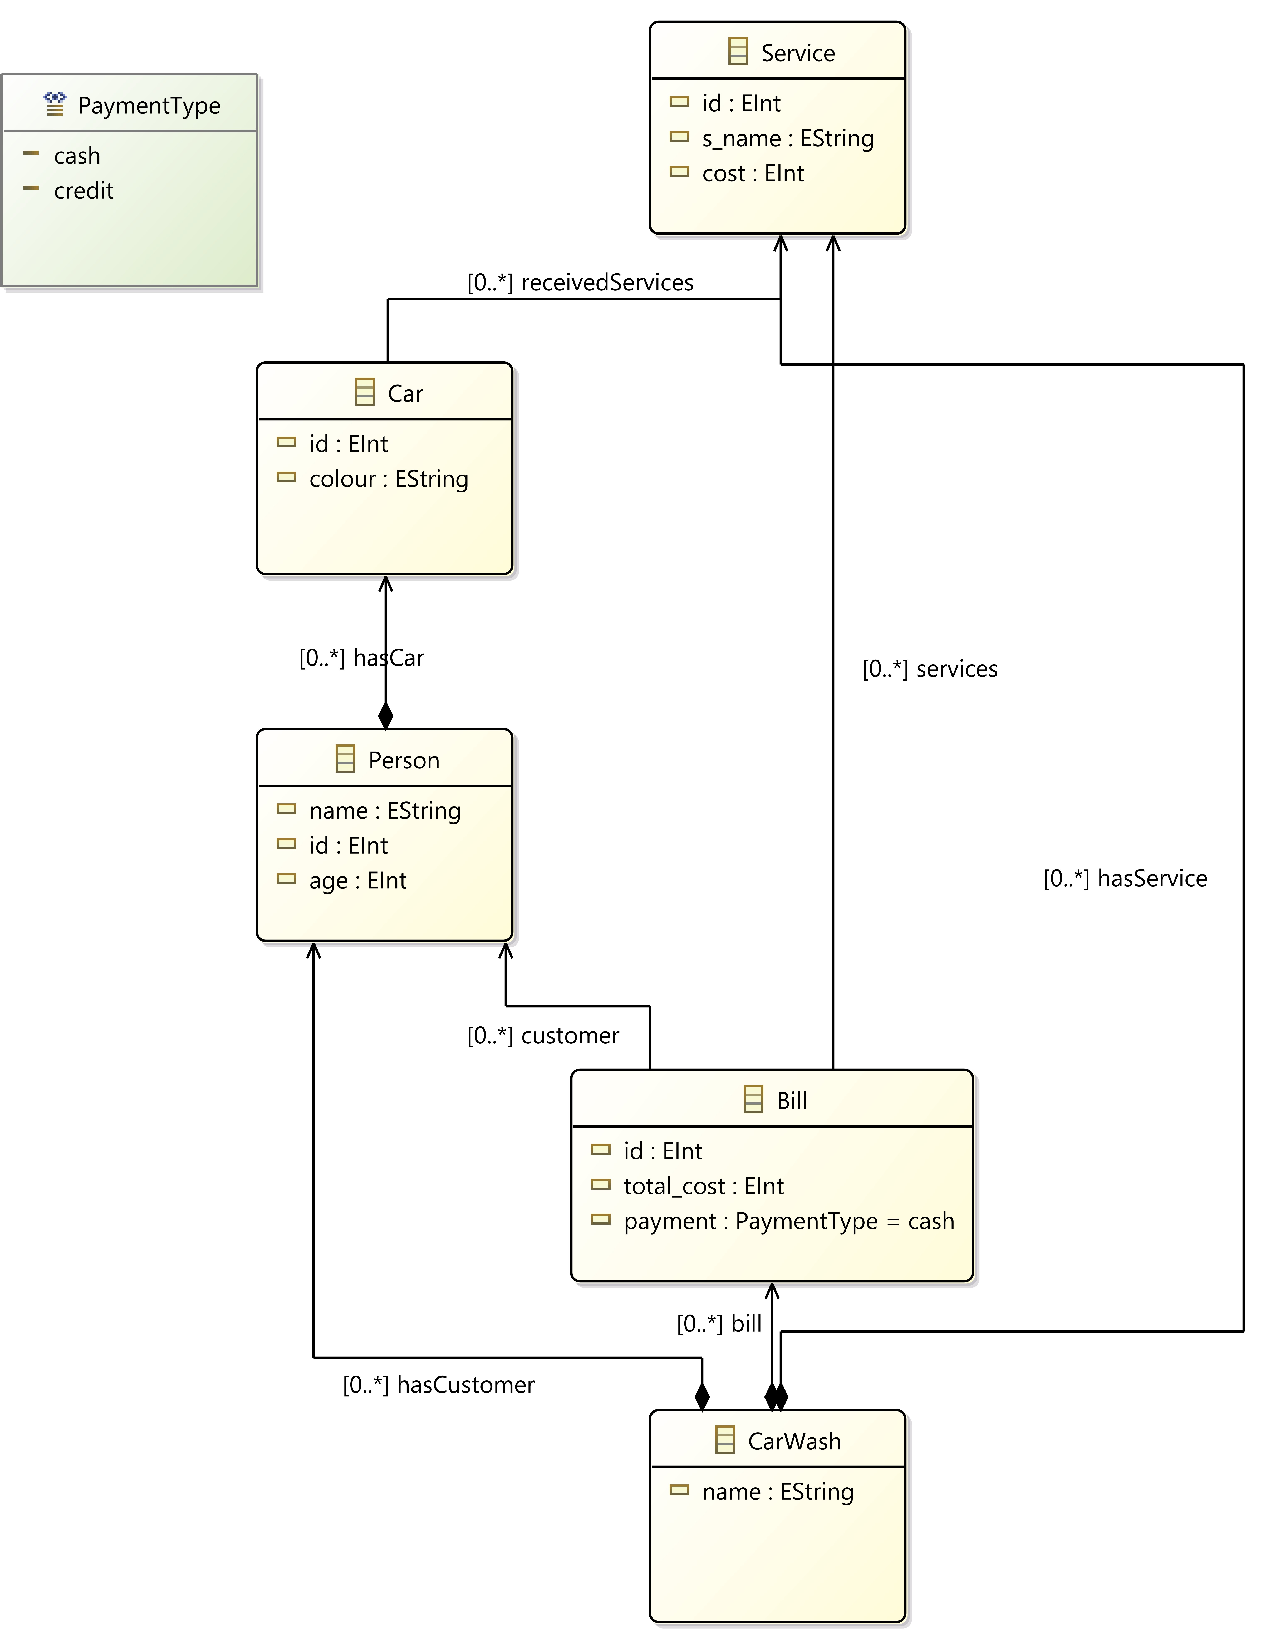
\includegraphics[width=10 cm, clip]{Figures/ecorecarwash.pdf}
    \caption{Carwash metamodel in~\cite{rahimi2023towards}.\label{fig:ecorecarwash}}
\end{figure}


\begin{program_}[H]
\footnotesize
\begin{verbatim}
{'directed': True, 'multigraph': True,
'graph': {}, 'nodes': [{'type': 'Bill', 'id': 0},
{'type': 'Bill', 'id': 1},
{'type': 'CarWash', 'id': 2},
{'type': 'Car', 'id': 3},
{'type': 'Car', 'id': 4},
{'type': 'Car', 'id': 5},
{'type': 'Person', 'id': 6},
{'type': 'Person', 'id': 7},
{'type': 'Service', 'id': 8},
{'type': 'Service', 'id': 9},
{'type': 'Service', 'id': 10}],
'links': [{'type': 'customer', 'source': 0,
'target': 6, 'key': 0},
{'type': 'services', 'source': 0,
'target': 8, 'key': 0},
{'type': 'services', 'source': 0,
'target': 10, 'key': 0},
{'type': 'customer', 'source': 1,
'target': 7, 'key': 0},
{'type': 'services', 'source': 1,
'target': 9, 'key': 0},
{'type': 'bill', 'source': 2,
'target': 0, 'key': 0},
{'type': 'bill', 'source': 2,
'target': 1, 'key': 0},
{'type': 'hasCustomer', 'source': 2,
'target': 6, 'key': 0},
{'type': 'hasCustomer', 'source': 2,
'target': 7, 'key': 0},
{'type': 'hasService', 'source': 2,
'target': 8, 'key': 0},
{'type': 'hasService', 'source': 2,
'target': 9, 'key': 0},
{'type': 'hasService', 'source': 2,
'target': 10, 'key': 0},
{'type': 'receivedServices', 'source': 3,
'target': 8, 'key': 0},
{'type': 'receivedServices', 'source': 4,
'target': 10, 'key': 0},
{'type': 'receivedServices', 'source': 5,
'target': 9, 'key': 0},
{'type': 'receivedServices', 'source': 5,
'target': 10, 'key': 0},
{'type': 'hasCar', 'source': 6,
'target': 3, 'key': 0},
{'type': 'hasCar', 'source': 7,
'target': 4, 'key': 0},
{'type': 'hasCar', 'source': 7,
'target': 5, 'key': 0}]}
\end{verbatim}
\caption{The graph data of Carwash instance model in~\cite{rahimi2023towards}.}
\label{Listing:NetworkXRahimi}
\end{program_}

\subsection{Experiment 3}
In this experiment, we compared the graph encoding capabilities of MoEGL with the approach presented by Miranda~\cite{miranda2024towards}, which used machine learning-backed methods to compute model views with Heterogeneous Graph Neural Networks (HGNNs). Miranda et al. aimed to simplify the integration of machine learning into Model-Driven Engineering (MDE) by encoding instance models conforming to an FSM metamodel into graphs using both NetworkX and Heterogeneous PyG. Their encoding approach was designed to automatically infer inter-model links while decoupling the contributions of view engineers and machine learning specialists.

\rev{Miranda et al.\ print one sample graph, reproduced as Listing~\ref{Listing:NetworkXJames}: 3 nodes of type Transition, 4 of type State, and 6 edges whose types are the pairs \texttt{(Transition, source, State)} and \texttt{(Transition, target, State)}. We compared that listing entry by entry. It is one 7-node example, and it is the only graph from this paper for which a reference listing exists.}

\rev{The MoEGL configuration for this encoding has 19 lines: it restricts the node classes to \texttt{Transition} and \texttt{State}, keeps only the \texttt{source} and \texttt{target} references of \texttt{Transition}, and encodes no attribute values. Table~\ref{tab:experimentations} is computed on a different file, the statecharts instance distributed with the authors' prototype. That file contains 101 objects, of which 100 are states or transitions, and 130 \texttt{source}/\texttt{target} links. It has no published reference graph, so the table reports its size and we do not call it a match to the 7-node listing. The configuration is in the replication package.}


\begin{program_}[H]
\footnotesize
\begin{verbatim}
{
  "nodes": [
    {"type": "Transition", "id": 0},
    {"type": "Transition", "id": 1},
    {"type": "Transition", "id": 2},
    {"type": "State", "id": 3},
    {"type": "State", "id": 4},
    {"type": "State", "id": 5},
    {"type": "State", "id": 6}
  ],
  "links": [
    {"type": ("Transition", "source",
    "State"), "source": 0, "target": 3},
    {"type": ("Transition", "target",
    "State"), "source": 0, "target": 4},
    {"type": ("Transition", "source",
    "State"), "source": 1, "target": 4},
    {"type": ("Transition", "target",
    "State"), "source": 1, "target": 5},
    {"type": ("Transition", "source",
    "State"), "source": 2, "target": 5},
    {"type": ("Transition", "target",
    "State"), "source": 2, "target": 6}
  ]
}
\end{verbatim}
\caption{The graph data of the FSM instance model in~\cite{miranda2024towards}.}
\label{Listing:NetworkXJames}
\end{program_}



\rev{Table~\ref{tab:experimentations} summarises the model datasets of the three experiments and the graphs MoEGL produces from them. All numbers are computed by the replication scripts from the actual runs. ``Objects'' and ``references'' are counted on the loaded models before any adaptation (every object, every set non-derived reference link); ``nodes'' and ``edges'' are counted on the encoded graphs. The difference between the two pairs of columns is exactly what the configuration removes: in Experiment~1, annotations, operations, parameters and generic types (and their links) are dropped, so 61.4 objects become 43.9 nodes; in Experiment~2 nothing is removed, so the numbers coincide; in Experiment~3 only states, transitions and their \texttt{source}/\texttt{target} links are kept. Attribute values are not part of these graphs because none of the three original encoders uses them; the goal here is to evaluate whether MoEGL can replicate existing structural encoders.}

\rev{The three encoders of prior work, written in Java and Python by three different groups, are each expressed by a MoEGL configuration of 14 to 29 lines. For Lopez et al., the only one of the three with a published reference corpus, the current loader reproduces every published graph (500 Ecore, 500 RDS, 369 Yakindu). This supports the claim that the encoding step can be delegated to a declarative configuration. The cost of doing so is quantified in Section~\ref{sec:evaluation}, and the effect of the two features those encoders do not have, heterogeneous graphs and attribute encoding, is measured in Section~\ref{sec:learning}.}

\begin{table}[H]
\caption{\rev{Datasets of the three experiments and the graphs produced by MoEGL (averages per model, computed from the actual runs; objects/references before adaptation, nodes/edges after encoding).}\label{tab:experimentations}}
\begin{adjustwidth}{-\extralength}{0cm}
\centering
\small
\begin{tabularx}{\fulllength}{lccccccc}
\toprule
\textbf{Experiment} & \textbf{Input} & \textbf{Models} & \textbf{Avg. objects} & \textbf{Avg. references} & \textbf{Avg. nodes} & \textbf{Avg. edges} & \textbf{Config. (LoC)} \\
\midrule
\rev{Exp. 1~\cite{lopez2022generating}} & \rev{ecore} & \rev{500} & \rev{61.4} & \rev{159.6} & \rev{43.9} & \rev{120.5} & \rev{29} \\
\rev{Exp. 2~\cite{rahimi2023towards}} & \rev{xmi}   & \rev{11}  & \rev{40.6} & \rev{139.4} & \rev{40.6} & \rev{139.4} & \rev{14} \\
\rev{Exp. 3~\cite{miranda2024towards}} & \rev{xmi}   & \rev{1}  & \rev{101.0} & \rev{266.0} & \rev{100.0} & \rev{130.0} & \rev{19} \\
\bottomrule
\end{tabularx}
\end{adjustwidth}
\end{table}


\subsection{Additional Experiment: Using Models in Graph-Learning Benchmarks}

In the main experimentation, we replaced existing encoders from the MDE community with MoEGL encoders. Here we focus on a well-known graph-learning benchmark from the ML community, based on a graph dataset. We show that the same ML task can be performed using a dataset of modeling artifacts and a MoEGL encoder. This way, we want to show that MoEGL enables tackling common graph learning problems using models.

We choose an existing graph dataset and create a metamodel representing the graphs. We programmatically translate graphs of the dataset into instances of such metamodel. We write a MoEGL configuration that encodes these models. Finally, we compare the result of the encoding to the original graphs in the dataset, aiming at obtaining the same graphs.
The AIDS dataset from TUDataset~\cite{morris2020tudataset} is chosen as it contains node/edge labels and attributes. The dataset contains 2000 virus-screening compound graphs. Each node contains attributes like position, charge, and a label for its symbol. There are 38 symbol types and 3 edge types. The AIDS metamodel in Figure~\ref{fig:aidsmetamodel} depicts the structure of the AIDS graphs.
The attribute values are stored in the node attributes vector. The model is converted to the NetworkX format using MoEGL. We compared the generated graph and the original graph and found that the encoded structure and attributes are the same.

We are aware that the experiment validity is hampered by a certain circularity (i.e. we create the metamodel and both the model-to-graph and graph-to-model transformation), but we believe it to be still a meaningful hint to the potential of broadening the applicability of MDE techniques to graph learning.

\begin{figure}[H]
    \centering
    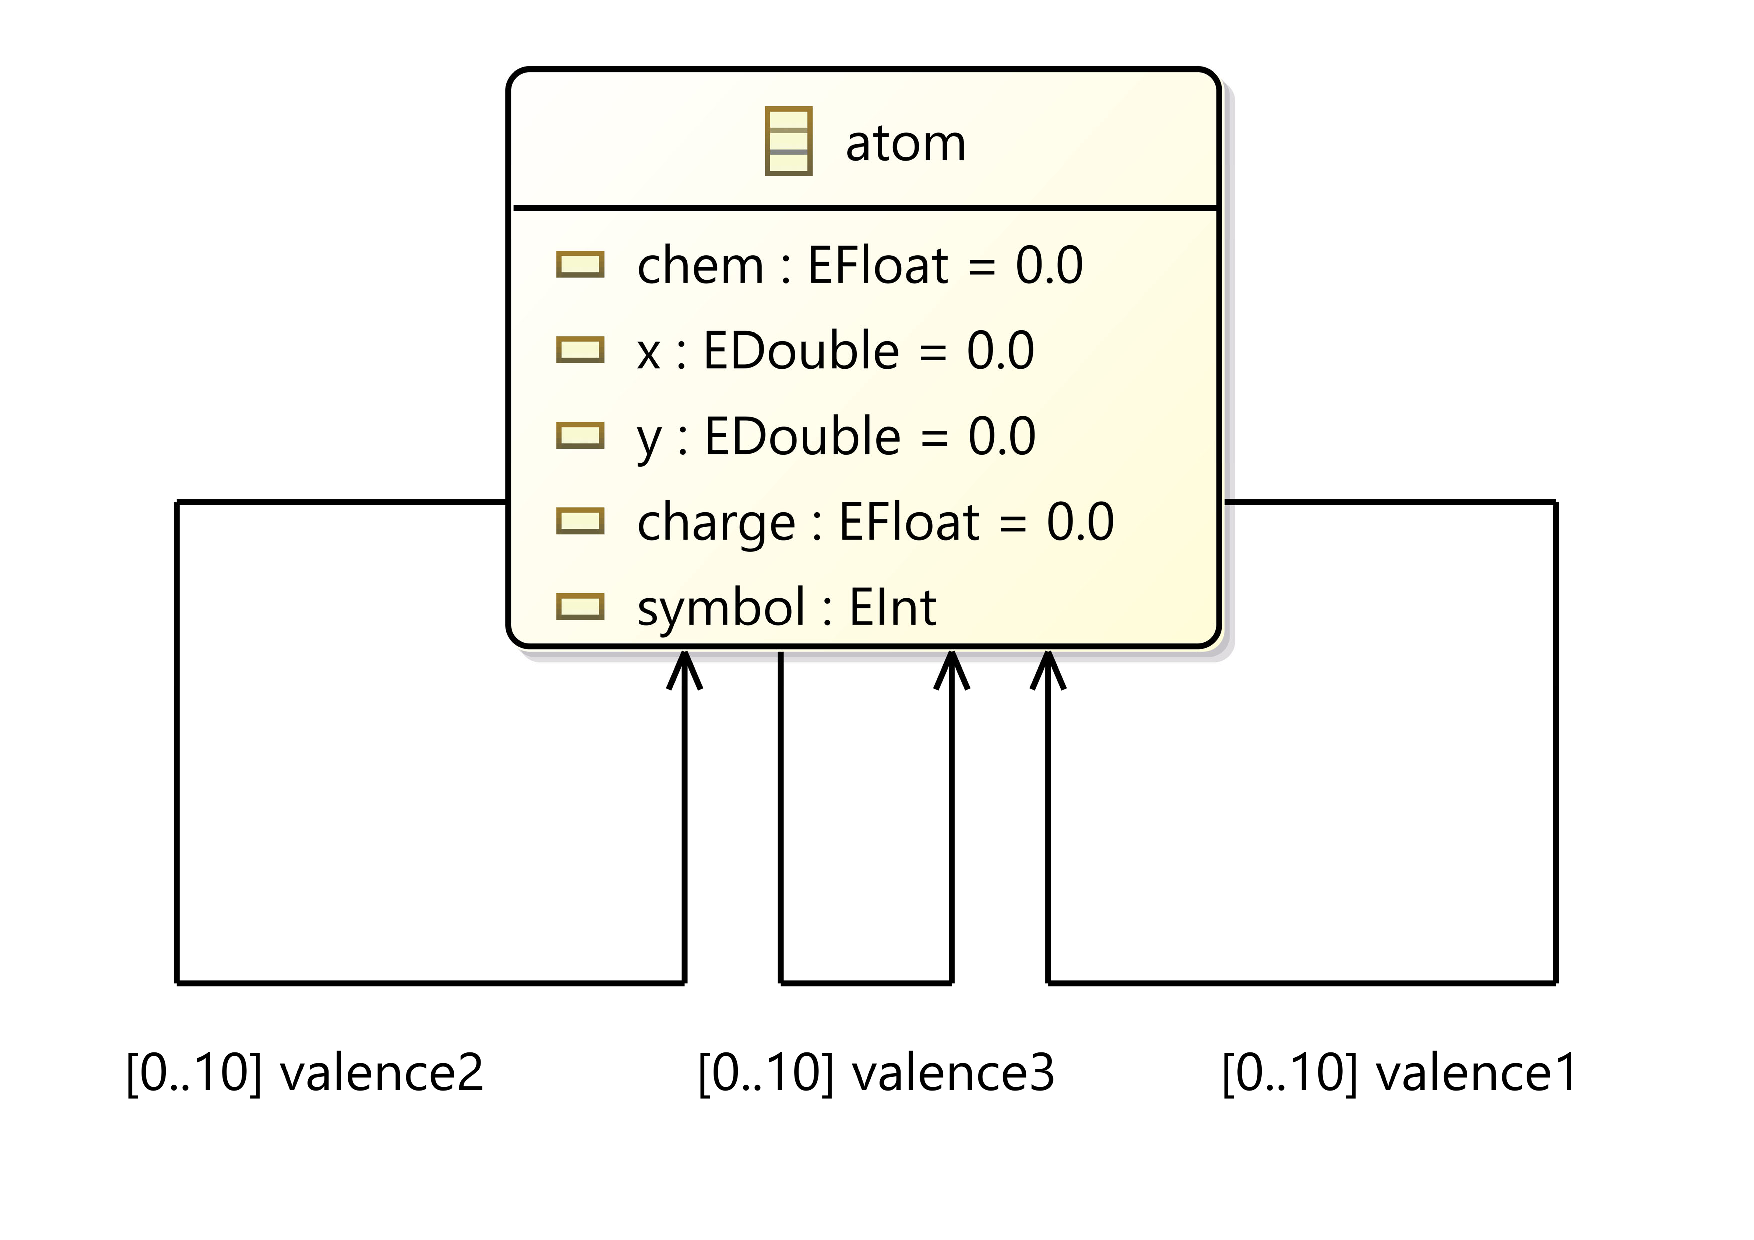
\includegraphics[width=10 cm]{Figures/AIDSmetamodel.pdf}
    \caption{The metamodel representing the graphs in the AIDS dataset.\label{fig:aidsmetamodel}}
\end{figure}

\subsection{Evaluation of MoEGL against Bespoke Encoders}\label{sec:evaluation}

\rev{This section quantifies the cost of using MoEGL instead of a hand-written encoder along three measurable dimensions, encoding time, peak memory and specification effort (lines of code), and states explicitly which properties we do \emph{not} measure. All numbers are produced by the scripts of the replication package and can be regenerated with one command.}

\subsubsection{\rev{Measurement Protocol}}

\rev{\textbf{Dataset.} The Ecore-GitHub dataset of Experiment~1: 500 real Ecore metamodels (21{,}938 objects in total), the only one of the three datasets for which the original encoder and its published output are available, so that fidelity, time and code size can all be measured on the same input.}

\rev{\textbf{Compared encoders.} (a) The bespoke encoder of Lopez et al.~\cite{lopez2022generating}, i.e., the authors' own Java implementation (EMF~2.20, JGraphT, Gson) executed unchanged through a 40-line driver that performs exactly the steps of their \texttt{GenerateRealGraphsEcore} program on the 500 files (resource loading, graph construction, JSON serialisation) without the corpus filtering and random sampling that precede them, since the released files already are the sampled set. (b) MoEGL with the configuration of Listing~\ref{code:yamlyakindu}, run as a Python process that performs Stage~1 (model loading with an lxml reader and extraction of objects and links into the cache) followed by Stage~2 (adaptation and NetworkX graph construction).}

\rev{\textbf{Timing.} Each measurement is the wall-clock time of the encoding loop inside the process (JVM or Python interpreter start-up excluded), measured with \texttt{System.nanoTime} and \texttt{time.perf\_counter}, respectively; we also report the total process time including start-up. Every configuration is executed in $N=10$ independent, freshly started processes and we report the mean and the sample standard deviation over the 10 runs. In addition, we measure MoEGL's \emph{re-encoding} time, i.e., Stage~2 alone starting from the Stage~1 cache with a second configuration (the same graph without data types and enumeration literals, and with class names encoded by word2vec), which is the situation of a user who iterates on the encoding of a fixed dataset. All runs were executed sequentially on an otherwise idle laptop: AMD Ryzen~9 4900H (8 cores/16 threads), 47~GB RAM, Windows~11 (build 26200), models on a local SSD, OpenJDK~21.0.3, Python~3.10.9, lxml, NetworkX~3.4.2, gensim~4.4.0.}

\rev{\textbf{Memory.} Peak memory was measured in a separate session, with the same two commands, the same 500 models and the same machine: ten fresh Java processes, then ten fresh MoEGL processes. Every 20~ms the process tree is sampled and the operating-system peak counters are read. Those counters are cumulative, so the value is the high-water mark of the worker, not a single instant. The worker is \texttt{java.exe} for the bespoke encoder. For MoEGL it is the base \texttt{python.exe} interpreter; the virtual-environment launcher only starts that interpreter and is not the measured process. Peak working set is \texttt{PeakWorkingSetSize}, the most physical memory resident in the worker. Peak committed memory is \texttt{PeakPagefileUsage}, the most memory the worker committed, which for the JVM includes heap that was not all resident. Both are reported in MB, where $1$~MB $=2^{20}$ bytes, as the mean and the sample standard deviation over the ten runs. The 47~GB figure is the installed RAM of the laptop, not the memory used by either encoder.}

\rev{\textbf{Lines of code.} Counted with \texttt{cloc}~2.06 (code lines only; blank and comment lines excluded). For the three bespoke encoders we count only the files that implement the model-to-graph encoding, taken from the authors' public repositories, and exclude training, generation and plotting code: for Lopez et al.\ the Java classes \texttt{Parser}, \texttt{GraphModel}, \texttt{MetaFilterLiterals}, \texttt{IMetaFilter} and the Python loader \texttt{json2graph.py} (409~LoC), plus the 190-LoC program that drives them; for Rahimi et al.~\cite{rahimi2023towards} \texttt{encoder.py} (249~LoC); for Miranda et al.~\cite{miranda2024towards} \texttt{to\_graph.py}, \texttt{encoders.py} and \texttt{metamodels.py} (193~LoC). For MoEGL we count the tool itself (655~LoC of Python, of which 68 are the command-line interface and 56 the optional HeteroData exporter) and, separately, the YAML configuration of each experiment.}

\subsubsection{\rev{Results}}

\begin{table}[H]
\caption{\rev{Encoding the 500 Ecore models of Experiment~1: fidelity, time and peak memory (mean $\pm$ sample standard deviation over $N=10$ fresh processes) and size of the specification. LoC counted with \texttt{cloc} (code lines only). Memory is in MB, with $1$~MB $=2^{20}$ bytes.}\label{tab:evaluation}}
\begin{adjustwidth}{-\extralength}{0cm}
\centering
\small
\begin{tabularx}{\fulllength}{lrr}
\toprule
& \textbf{Bespoke encoder~\cite{lopez2022generating} (Java)} & \textbf{MoEGL (Python)} \\
\midrule
\rev{Graphs identical to the published ones} & \rev{492 / 500$^{a}$} & \rev{500 / 500} \\
\midrule
\rev{Encoding time, in-process (s)} & \rev{$1.48 \pm 0.10$} & \rev{$1.11 \pm 0.02$} \\
\rev{\quad of which Stage 1: model loading and extraction} & \rev{--} & \rev{$0.67 \pm 0.01$} \\
\rev{\quad of which Stage 2: adaptation and graph construction} & \rev{--} & \rev{$0.45 \pm 0.01$} \\
\rev{Total process time incl.\ start-up (s)} & \rev{$2.01 \pm 0.12$} & \rev{$1.81 \pm 0.05$} \\
\rev{Peak working set (MB)$^{c}$} & \rev{$236.6 \pm 10.1$} & \rev{$153.5 \pm 0.2$} \\
\rev{Peak committed memory (MB)$^{c}$} & \rev{$957.0 \pm 10.8$} & \rev{$624.6 \pm 0.3$} \\
\rev{Re-encoding from cache with a second configuration (s)} & \rev{n/a (full re-run)} & \rev{$1.16 \pm 0.33$~$^{b}$} \\
\midrule
\rev{Code written once (tool), LoC} & \rev{409 (+190 driver)} & \rev{655} \\
\rev{Code written per encoding task, LoC} & \rev{409 (+190 driver)} & \rev{29 (YAML)} \\
\bottomrule
\end{tabularx}
\end{adjustwidth}
\noindent{\small \rev{$^{a}$ The authors' code re-run on the released files; 8 released files reference themselves under their original name and load with unresolved links. $^{b}$ Includes training a word2vec model on all class names; with the original configuration Stage~2 alone takes $0.45 \pm 0.01$~s. $^{c}$ Separate session from the times, same commands. Peak working set is \texttt{PeakWorkingSetSize} of \texttt{java.exe} or of MoEGL's \texttt{python.exe}. Peak committed memory is \texttt{PeakPagefileUsage}. The process tree was sampled every 20~ms; the counters are cumulative.}}
\end{table}

\rev{\textbf{Fidelity.} The timed loader is the current one. An edge-preserving bijection matches 500 of 500 Ecore graphs, 500 of 500 RDS graphs and 369 of 369 Yakindu graphs (Section~\ref{Sec:Experiments}, Experiment~1). The graphs timed here are the same graphs as that certificate: after the loader changes in this section, the multiset of typed nodes and edges on the 500 Ecore models was unchanged. An earlier PyEcore loader matched 495 of 500.}

\rev{\textbf{Time.} On a first complete run the current loader is slightly faster than the bespoke Java encoder: $1.11 \pm 0.02$~s against $1.48 \pm 0.10$~s for the same 500 models, about 2.2~ms per model against 3.0~ms. Stage~1, which reads the files with lxml, takes $0.67 \pm 0.01$~s and Stage~2 takes $0.45 \pm 0.01$~s. In this session every one of the ten MoEGL runs (1.09--1.14~s) was faster than every Java run (1.36--1.68~s). An earlier PyEcore loader took $7.98 \pm 0.11$~s on the same task, of which $7.58$~s was Stage~1; that loader is not the one timed in Table~\ref{tab:evaluation}. Re-encoding from the cache, including a word2vec fit, takes $1.16 \pm 0.33$~s, while the Java encoder re-parses every model on each change. Both times remain small next to training a GNN on the resulting graphs.}

\rev{\textbf{Memory.} In the memory session the Java worker reached a peak working set of $236.6 \pm 10.1$~MB and a peak committed size of $957.0 \pm 10.8$~MB. The MoEGL interpreter reached $153.5 \pm 0.2$~MB resident and $624.6 \pm 0.3$~MB committed. Each figure is the high-water mark of one process that encodes all 500 models. It is not a per-model cost, and it is not the 47~GB of RAM installed on the machine. The committed size is larger than the working set because both runtimes commit memory that is not all resident at the peak; the gap is wider for the JVM.}

\rev{\textbf{Specification effort.} A fair comparison must account for the fact that MoEGL itself is code: 655 lines of Python that are written once and shared by all encoding tasks, against 409 (or 599 with the driver) lines for the one bespoke encoder we could measure in full, 249 and 193 lines for the two others. The difference lies in the cost \emph{per task}: each of the three encoders of prior work is expressed by 14 to 29 lines of YAML (Table~\ref{tab:experimentations}), and a new encoding for the same models is a change of a few lines in that file. The claim we make is therefore not that MoEGL removes code, but that it moves the code from every project into one reusable tool, so that the per-task effort drops from a few hundred lines of Java or Python, which require knowledge of EMF or PyEcore and of the graph library, to a few dozen declarative lines that only require knowledge of the metamodel.}

\subsubsection{\rev{Design Properties}}

\rev{Scalability, ease of use, maintainability and extensibility follow from the architecture, alongside the measurements above. \emph{Scalability:} the two-stage design builds the cache of a repository once and re-uses it; on the 500-model set the loader reads the models in $0.67$~s. \emph{Ease of use:} a configuration names classes and features in the metamodel's own terms, in 14 to 29 lines of YAML. \emph{Maintainability and extensibility:} a new encoding is an edit of that file, and a new value encoder is one function in the encoder module. A study with practitioners, and a timing series on corpora larger than these 500 models, are future work.}

\subsubsection{\rev{Threats to Validity}}

\rev{\emph{Construct validity.} Lines of code is an imperfect proxy for effort; it does not capture the time needed to learn a tool or the difficulty of the code. We mitigate this by counting only code lines, by applying the same tool and rules to all artefacts, and by reporting the size of MoEGL itself rather than only the configurations. The isomorphism test compares graphs with node and edge types only, which is exactly the information the compared encoders produce. \emph{Internal validity.} Timing compares a Java and a Python implementation and therefore also reflects language and library differences (EMF versus the lxml loader); we separate the loading stage from the DSL-driven stage to make this visible and we report both in-process and total process time over ten fresh runs. The memory figures have the same limit: they are the peak of the whole worker process, including the JVM or the Python interpreter, not the graph alone. The memory session is separate from the timing session. \emph{External validity.} The timed comparison uses one dataset and one bespoke encoder. The edge-preserving certificate additionally covers the published RDS and Yakindu graphs. The two other encoders are compared on code size and on small datasets (11 and 1 models). The classification result is for one task and one near-duplicate split; it does not transfer automatically to other MDE tasks, and our split is not the unpublished duplicate list of Lopez et al.~\cite{lopez2022classification}. Behaviour on very large instance models has not been measured. We have not checked whether names from this ModelSet split occur in the corpus on which WordE4MDE was trained. The balanced accuracies $0.808$ and $0.824$ in Section~\ref{sec:learning} are the TF-IDF SVM and the relation-token SVM. \emph{Reliability.} All scripts, configurations, the compiled driver for the bespoke encoder, the raw timing samples and the per-model comparison results are available in the replication package, together with the exact software versions used.}

\rev{\textbf{Robustness of a downstream learner.} Tahmasivand et al.~\cite{tahmasivand2025lmfix} detect and recover bit-flips inside a language model. Zahran et al.~\cite{zahran2025jailbreak} jailbreak quantized language models by injecting faults into their weights. Omidi et al.~\cite{omidi2026undervolting} measure the adversarial accuracy of convolutional networks trained on an undervolted GPU. These three studies concern hardware faults in language models and convolutional networks. None of them takes an EMF model or a MoEGL graph as input. This article does not measure bit-flip detection, jailbreaks under fault injection, or adversarial robustness under undervolting. The reliability it reports is the edge-preserving reproduction of the published graphs (Section~\ref{Sec:Experiments}) and the split protocol of Section~\ref{sec:learning}.}


\subsection{\rev{Effect of the Encoding on Model Classification}}\label{sec:learning}

\rev{Experiments~1--3 encode no attribute values, because the encoders they replicate do not. The two features that go beyond those encoders are heterogeneous graphs and attribute encoding. We measure them on domain classification of Ecore metamodels, the task of Lopez et al.~\cite{lopez2022classification}.}

\rev{\textbf{Data and protocol.} From ModelSet~\cite{lopez2022modelset} we keep categories with at least ten models, drop the labels dummy and unknown, and remove near-duplicates: within a category, models whose identifier tokens have Jaccard similarity at least 0.8 are collapsed. The resulting set has 2{,}074 models and 48 categories. Lopez et al.\ report a no-duplicate split of 2{,}068 models and 48 categories; our file list is not theirs, so we compare methods on our split and cite their published numbers only as context. The metric is balanced accuracy, the average of the per-category recalls. Evaluation is stratified 5-fold cross-validation repeated with two seeds. Inside each training fold, 15\% of each category is a validation slice. The SVM regularisation $C\in\{0.1,1,10\}$ and the GNN epoch are chosen on that slice; the test fold is scored once. A GNN trains for at most 30 epochs and stops after 6 epochs with no improvement of the validation balanced accuracy. The epoch with the highest validation score is the one applied to the test fold. Class weights are balanced.}

\rev{\textbf{Encodings.} All graphs are produced by MoEGL. The name baseline is a TF-IDF vector of the element-name tokens and a linear SVM, the family of the strongest published result on this task. The MoEGL relational encoding appends tokens the bag of names cannot see, one per structural feature (\texttt{owner>kind:lower-upper>type}, with kind attribute, containment or reference) and one per named typed edge. The GNN comparison holds the node features fixed as the mean WordE4MDE vector of each element's name~\cite{lopez2023word} and changes only the graph: a homogeneous GIN, which ignores edge types, against a heterogeneous RGCN, which uses them. A third RGCN adds the numeric structural attributes (abstract, interface, containment, bounds and the related flags) to those name vectors.}

\rev{\textbf{Embedding fit and the split.} Table~\ref{tab:learning} does not use the dataset-wide word2vec fit of Section~\ref{sec:avalues}. The TF-IDF vectorizer is fitted on the training indices of each fold and then applied to the validation slice and the test fold. The relation tokens are read from the metamodel. The GNN node features are a lookup in the frozen WordE4MDE table, which is not estimated on this split.}

\begin{table}[H]
\caption{\rev{Domain classification on the near-duplicate ModelSet split (2{,}074 models, 48 categories). Balanced accuracy, mean $\pm$ sample standard deviation over 10 test folds. Model selection uses the validation slice only.}\label{tab:learning}}
\centering
\small
\begin{tabular}{llc}
\toprule
\textbf{Encoding} & \textbf{Model} & \textbf{Balanced accuracy} \\
\midrule
\rev{Element names (TF-IDF)} & \rev{Linear SVM} & \rev{$0.808 \pm 0.024$} \\
\rev{Names plus MoEGL relation tokens} & \rev{Linear SVM} & \rev{$0.824 \pm 0.025$} \\
\rev{WordE4MDE name on each node, untyped edges} & \rev{GIN} & \rev{$0.770 \pm 0.029$} \\
\rev{Same node features, typed edges} & \rev{RGCN} & \rev{$0.795 \pm 0.036$} \\
\rev{Typed edges plus numeric attributes} & \rev{RGCN} & \rev{$0.782 \pm 0.040$} \\
\bottomrule
\end{tabular}
\end{table}

\rev{On our split, Lopez et al.~\cite{lopez2022classification} cannot be re-scored model by model, because their duplicate list is not public. On their own no-duplicate split they report balanced accuracy 0.825 for a feed-forward network on TF-IDF names, 0.816 for an SVM on the same names, and 0.808 for a GNN on the raw graph. Our relational SVM reaches 0.824. That is level with their best published name classifier and above both their SVM and their GNN. The splits differ, so this is a comparison of published figures, not a claim that we have exceeded 0.825 on their files.}

\rev{\textbf{What the two features do.} The relation tokens are the part of the result that the DSL adds. They raise balanced accuracy by $0.016$ over names alone (standard deviation of the ten paired differences $0.017$; paired $t=2.93$, $p=0.017$; better on 8 of the 10 folds). With the name vector of each node held fixed, the heterogeneous RGCN scores $0.795\pm0.036$ and the homogeneous GIN $0.770\pm0.029$. The mean of the ten paired differences is $0.025$ (standard deviation $0.037$; paired $t=2.14$, two-sided $p=0.061$; the RGCN is higher on 7 of the 10 folds). The same training was repeated with the validation score stored after every epoch, and the test scores reproduced Table~\ref{tab:learning}. The selected epoch is $16.4\pm3.8$ for the GIN and $15.2\pm4.7$ for the RGCN. Training then continues until the patience limit, for $22.4\pm3.8$ and $21.2\pm4.7$ epochs. Validation balanced accuracy at the selected epoch is $0.810\pm0.042$ for the GIN and $0.822\pm0.042$ for the RGCN. On the first 15 epochs, the longest prefix reached by every fold, the mean validation score of the RGCN is higher at every epoch (0.398 against 0.165 after epoch~1). The typed graph raises the score that training reaches, at a similar number of epochs. Numeric structural attributes do not add a further gain; that RGCN scores $0.782$. The useful attribute on this task is the element name. A linear SVM on the mean WordE4MDE vector of the whole model, with no graph, scores \(0.808\pm0.024\), level with TF-IDF names (Section~\ref{sec:avalues}), so the pre-trained name vectors are available when a dataset is too small to fit word2vec. The learning claim is therefore specific: the relational graph reaches the level of the best published name classifier and is a small, statistically detectable improvement on a bag of names; the numeric flags are not what produces that score.}

\subsection{\rev{Scope of a Configuration}}\label{sec:limits}
\rev{The language selects classes and features, renames them, and encodes attribute values that stay on their element. The three graph encoders of Experiments~1--3 sit inside that selection. The operations below stay outside it.}
\begin{itemize}
    \item \rev{\textbf{An attribute does not become a node.} A value such as \texttt{State.name} is stored on the State node. There is no construct that replaces the attribute with a node of its own. Making the value a node requires the value to be an object in the metamodel.}
    \item \rev{\textbf{A reverse edge follows the opposite declared on the feature.} When a feature records an opposite, and that opposite feature exists on the target class and is not derived, the loader writes the reverse edge under the opposite's name. On the Ecore metamodel used here, \texttt{EReference.eOpposite} records no opposite, so that edge is written only where the file serializes it. Section~\ref{sec:semantics} states the rule. There is no key that inserts any further edge.}
    \item \rev{\textbf{An edge has no feature vector.} The edge stores the reference name in its \texttt{type}. Attribute encodings (\texttt{RawString}, \texttt{one-hot}, \texttt{word2vec}, \texttt{worde4mde}) apply to values on nodes. A reference such as \texttt{eType} therefore remains an edge, which is why Listing~\ref{code:yamlecoreAttribute} encodes \texttt{name} and \texttt{abstract} and does not attach an encoding to \texttt{eType}. In the NetworkX writer the key \texttt{type} is the class name, so a feature that is itself named \texttt{type} makes that writer raise an error. The heterogeneous output keeps the class as the node type and puts the value in the feature tensor, as in Listing~\ref{fig:outputFSM}.}
\end{itemize}
\rev{Table~\ref{tab:coverage} places the published encoders we considered on this boundary. The three graph encoders of Experiments~1--3 are configurations of MoEGL. A graph kernel and a tree-to-sequence encoding are not configurations of MoEGL: the tool stops once the graph is written.}

\begin{table}[H]
\caption{\rev{Encoders MoEGL reproduces, and encodings it does not produce.}\label{tab:coverage}}
\centering
\small
\begin{tabularx}{\textwidth}{lXX}
\toprule
\textbf{Encoder} & \textbf{What it produces} & \textbf{MoEGL} \\
\midrule
\rev{Lopez et al.~\cite{lopez2022generating}} & \rev{Typed nodes and references, no attribute values} & \rev{Reproduced: 500/500 Ecore, 500/500 RDS, 369/369 Yakindu} \\
\rev{Rahimi et al.~\cite{rahimi2023towards}} & \rev{Class as node type and reference name as edge type, then an untyped symmetric matrix for NetGAN} & \rev{The 14-line configuration produces the typed graph. The matrix step that drops direction and edge labels is theirs} \\
\rev{Miranda et al.~\cite{miranda2024towards}} & \rev{Transition and State nodes, \texttt{source} and \texttt{target} edges} & \rev{The printed 7-node graph matches entry by entry. The 100-node file has no published graph} \\
\rev{Claris\'o and Cabot~\cite{clariso2018applying}} & \rev{A graph kernel over models} & \rev{Not produced. MoEGL writes the graph and does not compute a kernel} \\
\rev{Burgue\~no et al.~\cite{burgueno2019lstm}} & \rev{A containment tree read as a sequence by an LSTM} & \rev{Not produced. MoEGL does not emit that sequence} \\
\bottomrule
\end{tabularx}
\end{table}

\section{Related Work} \label{Sec:relatedwork}
This section reviews some related studies that are proposed to do MDE tasks using ML models, especially those that exploit the model-to-graph encoding. \rev{MoEGL is not the first encoding of models as graphs. L\'opez et al., Rahimi et al.\ and Miranda et al.\ each wrote an encoder for one corpus, and a workshop paper proposed a DSL for homogeneous graphs~\cite{rajaei2021dsl}. The addition here is one configuration language for those encodings, together with heterogeneous graphs and attribute values. The tool writes NetworkX graphs and PyTorch Geometric heterogeneous graphs~\cite{fey2019fast}. The Deep Graph Library~\cite{wang2019deep} is another general graph-learning library, and MoEGL does not emit it. The classification experiment uses the Ecore models of ModelSet~\cite{lopez2022modelset}.}


ML algorithms have effectively tackled various challenges in MDE~\cite{babur2018ammore}. For instance, model transformation rules were automatically inferred from sets of source and target models using ML techniques in~\cite{burgueno2019lstm, dolques2010learning}. In~\cite{babur2016hierarchical}, a set of metamodels is arranged using hierarchical clustering to produce meaningful visualizations. Hierarchical clustering is also used in~\cite{basciani2016automated} to organize the models employing the MDEForge tool. There has also been a discussion on model encoding for clustering in~\cite{babur2017using}.
Nguyen et al.~\cite{nguyen2019automated} introduce a classification of metamodels by a tool implementing a feed-forward neural network. They propose some preprocessing tasks to transform a metamodel into a feature vector. The tasks consist of a term extractor that parses the terms in the meta-model, and then of an NLP Normalizer that normalizes the extracted terms by performing some Natural Language Processing (NLP) tasks. Burgueno et al.~\cite{burgueno2019lstm} propose a neural network architecture based on Long Short-Term Memory (LSTM) Neural Networks to perform model transformation automatically. They propose to apply a preprocessing method to represent models as trees before feeding them to an Artificial Neural Network (ANN). After transforming the model into a tree using the proposed strategy, a normalization process is applied to overcome the limitations of ANNs. Couto et al.~\cite{couto2020classifying} propose to classify unstructured models into meta-models using Multi-Layer Perceptrons (MLP). They translate a meta-model containing classes, attributes, and references into a set of name/value pairs in a JSON format. Then a binary vector is created as the MLP's input feature.

Some studies use model-to-graph encoding as their encoding approach. López et al.~\cite{lopez2021towards} address the issue of determining a generator's level of realism. They map it to a classification task where a GNN will be trained to discriminate between the two sets of models (real and synthetic). In another study, López et al.~\cite{lopez2022generating} propose a new architecture for the design of structurally realistic generators. This kind of generator can create new models that are essentially novel but structurally similar to the models in the dataset given a dataset that includes multiple models considered real models. Graph kernels are suggested to be applied to MDE by the authors in~\cite{clariso2018applying}. Accordingly, Di Rocco et al.~\cite{di2021gnn} suggest MORGAN, a graph kernel-based tool to assist in the completion of models and metamodels. The tool's idea is to suggest structural elements to finish the models that are currently being built. Specifically, MORGAN can suggest metaclasses, structural elements like attributes and references, and classes, fields, and methods inside a model class.
Rahimi et al.~\cite{rahimi2023towards} utilize generative adversarial networks (GANs) to automatically generate new structurally realistic models from a metamodel and instance model. The proposed GAN-based tool is built on the Eclipse Modeling Framework. Graph metrics are used to evaluate whether the generated artificial models match the properties of the original example model.
Miranda et al.~\cite{miranda2024towards} introduced the concept of model views to integrate heterogeneous models in MDE, the ViewPoint Definition Language (VPDL) for specifying model views, and the EMF Views solution. They have used an ML approach introduced to support automated link inference and HGNNs as the ML technique.

Clarisó and Cabot's work~\cite{clariso2022user} on user-driven diverse scenario exploration in model finders presents a domain-specific language (DSL) aimed at controlling how Alloy specifications are encoded into graphs for clustering purposes. Their DSL allows users to define scenarios by selecting and filtering model elements and attributes, providing a flexible approach to model exploration and analysis. This method, while targeting Alloy specifications, demonstrates the broader applicability and influence of DSLs in model-driven engineering. The concepts of selecting and filtering elements in their DSL are closely aligned with our approach, emphasizing the importance of user control and customization in model encoding processes. This highlights the versatility of DSLs in enhancing the usability and precision of model-driven tasks.

\rev{Each of those encoders is written for one task. MoEGL expresses the three graph encoders of Section~\ref{Sec:Experiments} by a configuration of 14 to 29 lines. The learning task measured here is domain classification: relation tokens raise balanced accuracy from $0.808$ to $0.824$.}

\rev{Five publications from 2025 and 2026 still depend on a representation of the model. L\'opez et al.~\cite{lopez2025modelxglue} separate encoding from training in a benchmark harness, and record that a GNN requires the models in a graph format. L\'opez et al.~\cite{lopez2025worde} extend the WordE4MDE vectors with subword units, a BERT model trained on modelling text, and additional forum text. Section~\ref{sec:learning} uses the skip-gram vectors of the 2023 paper~\cite{lopez2023word}. Khalilipour et al.~\cite{khalilipour2025retrieval} turn each Ecore metamodel into a semantic attributed graph and classify it with a GNN into 24 categories, using BERT or TF-IDF features. They report an accuracy of about 96\% for the BERT model on that retrieval task. The category set, the metric and the features differ from Section~\ref{sec:learning}. Chen et al.~\cite{chen2025graphgen} generate a graph model from text so that the result satisfies a metamodel. Ali~\cite{ali2026symbols} encodes Ecore, OntoUML and ArchiMate models as knowledge graphs and trains a GNN together with a language model. These works consume a graph or a name vector. The configuration that chooses the graph is the subject of this article.}

\subsection{Domain-Specific Transformation Languages (DSTLs)}
\rev{Csert\'an et al.~\cite{csertan2002viatra} presented VIATRA, a language that transforms a model into another model for verification. Varr\'o is a co-author of that paper. MoEGL does not transform a model into another model. It writes a graph for a learner.}


\section{Evaluation of Research Contributions and Questions}
\rev{Each question is answered in the experiment that measures it. The figures are stated there, and they are not copied here.}
\begin{itemize}
    \item \rev{\textbf{RQ1 (Fidelity).} Experiment~1 (Section~\ref{Sec:Experiments}) compares the MoEGL graphs with the published graphs.}
    \item \rev{\textbf{RQ2 (Cost).} Section~\ref{sec:evaluation} and Table~\ref{tab:evaluation} report specification size, encoding time and peak memory.}
    \item \rev{\textbf{RQ3 (Effect).} Section~\ref{sec:learning} and Table~\ref{tab:learning} report the classification result, including the homogeneous and heterogeneous models.}
\end{itemize}
\rev{Together these three results are the evaluation of the contribution. The boundary of the language is Section~\ref{sec:limits}.}


\section{Conclusion and Future Work} \label{Sec:conclusion}

In this paper, we introduced MoEGL, a domain-specific language designed to encode models into graphs compatible with graph neural networks. \rev{One configuration reproduces the published graphs of L\'opez et al.\ (500 Ecore, 500 RDS, 369 Yakindu), the per-task specification is 14 to 29 lines of YAML, and relation tokens raise balanced accuracy from $0.808$ to $0.824$ on domain classification.} Future work will explore further enhancements to MoEGL and its application to other MDE tasks.

\rev{The work sits next to the encoders of L\'opez et al., Rahimi et al.\ and Miranda et al., and next to the 2021 workshop DSL. What this article adds, and measures, is one shared configuration for those encodings, heterogeneous graphs, attribute-value encodings, and the classification result in Section~\ref{sec:learning}.}

Looking ahead, we aim to apply MoEGL to further learning tasks on models. Some potential avenues of future work include considering alternate encodings for attribute values within MoEGL, allowing users to filter model elements according to Object Constraint Language (OCL) expressions defined in the MoEGL configuration, and more fully realizing the proposed heterogeneous graph encoding approach. A goal is to semantically encode the element names in models to facilitate various MDE activities. Another possible extension of this research going forward involves designing heuristics to automatically determine well-suited encodings based on analyzing a metamodel's structure and characterizing the ML objective. Moving ahead, we plan to extensively research the applicability of encoding models as heterogeneous graphs for a wide range of MDE use cases. We also intend to support other popular GNNs and HGNNs like the new implementation of heterogeneous graphs in tensorflow~\cite{HPyG_Tensorflow}.

%%%%%%%%%%%%%%%%%%%%%%%%%%%%%%%%%%%%%%%%%%
\vspace{6pt}

%%%%%%%%%%%%%%%%%%%%%%%%%%%%%%%%%%%%%%%%%%
%% optional
%\supplementary{The following supporting information can be downloaded at \linksupplementary{s1}, Figure S1: title; Table S1: title; Video S1: title.}

%%%%%%%%%%%%%%%%%%%%%%%%%%%%%%%%%%%%%%%%%%
\authorcontributions{Conceptualization, Z.R. and S.K.-R.; methodology, Z.R.; software, Z.R.; validation, Z.R., S.K.-R. and M.T.; formal analysis, Z.R.; investigation, Z.R.; resources, Z.R.; data curation, Z.R.; writing---original draft preparation, Z.R.; writing---review and editing, S.K.-R. and M.T.; visualization, Z.R.; supervision, S.K.-R. and M.T.; project administration, S.K.-R.; funding acquisition, S.K.-R. All authors have read and agreed to the published version of the manuscript.}

\funding{This research received no external funding.}

\institutionalreview{Not applicable.}

\informedconsent{Not applicable.}

\dataavailability{The source code of MoEGL, the configurations of the three experiments, the measurement scripts (fidelity check, timing, lines-of-code count), the driver used to run the bespoke encoder of Experiment~1 and the raw results are openly available in the MoEGL repository at \url{https://github.com/Z-Rajaei/MoEGL}. \rev{The running-example metamodel, instance and the four YAML listings are in \texttt{examples/running\_fsm}, and \texttt{examples/running\_fsm/check\_listings.py} is the script that executed them.} \rev{The 500 Ecore models and the published graphs of Experiment~1 are part of the replication package of Lopez et al.\ (TCRMG-GNN, \url{https://github.com/Antolin1/TCRMG-GNN}).}}

\acknowledgments{During the preparation of this manuscript, the authors used generative AI tools (e.g., ChatGPT and GitHub Copilot) for language polishing and code assistance. The authors have reviewed and edited the output and take full responsibility for the content of this publication.}

\conflictsofinterest{The authors declare no conflicts of interest. The funders had no role in the design of the study; in the collection, analyses, or interpretation of data; in the writing of the manuscript; or in the decision to publish the results.}

%%%%%%%%%%%%%%%%%%%%%%%%%%%%%%%%%%%%%%%%%%
%% Optional
\abbreviations{Abbreviations}{%
The following abbreviations are used in this manuscript:\\

\noindent
\begin{tabular}{@{}ll}
MDE & Model-Driven Engineering\\
DSL & Domain-Specific Language\\
GNN & Graph Neural Network\\
HGNN & Heterogeneous Graph Neural Network\\
ML  & Machine Learning\\
AI  & Artificial Intelligence\\
EMF & Eclipse Modeling Framework\\
UML & Unified Modeling Language\\
XMI & XML Metadata Interchange\\
OCL & Object Constraint Language\\
GAN & Generative Adversarial Network\\
LSTM & Long Short-Term Memory\\
MLP & Multi-Layer Perceptron\\
NLP & Natural Language Processing\\
MoEGL & Model Encoding for Graph Learning\\
HPyG & Heterogeneous PyTorch Geometric\\
GCN & Graph Convolutional Network\\
GAT & Graph Attention Network\\
LoC & Lines of Code\\
DOI & Digital Object Identifier\\
CSV & Comma-Separated Values\\
FSM & Finite State Machine\\
URI & Uniform Resource Identifier\\
URL & Uniform Resource Locator\\
YAML & YAML Ain't Markup Language
\end{tabular}
}

%%%%%%%%%%%%%%%%%%%%%%%%%%%%%%%%%%%%%%%%%%
%% Optional
\begin{adjustwidth}{-\extralength}{0cm}

\reftitle{References}

%=====================================
% References, variant A: external bibliography
%=====================================
\bibliography{sn-bibliography}

%=====================================
% References, variant B: internal bibliography
%=====================================
% To use the internal bibliography, comment out the \bibliography line above
% and uncomment the thebibliography environment below, then add your bibitems.

%%%%%%%%%%%%%%%%%%%%%%%%%%%%%%%%%%%%%%%%%%
\PublishersNote{}
\end{adjustwidth}
\end{document}
